% !TEX TS-program = pdflatex
% !TEX encoding = UTF-8 Unicode

\documentclass[11pt,oneside]{book}
\usepackage[utf8]{inputenc} 
\usepackage[parfill]{parskip}
\usepackage[T1]{fontenc} 

\usepackage{fixltx2e}
\usepackage{calc}
\usepackage{doxygen}
\usepackage[export]{adjustbox} % also loads graphicx
\usepackage{makeidx}
\usepackage{multicol}
\usepackage{multirow}
\PassOptionsToPackage{warn}{textcomp}
\usepackage{textcomp}
\usepackage[nointegrals]{wasysym}
\usepackage[table]{xcolor}

% Font selection
\usepackage[T1]{fontenc}
\usepackage[scaled=.90]{helvet}
\usepackage{courier}
\usepackage{amssymb}
\usepackage{sectsty}
\renewcommand{\familydefault}{\sfdefault}
\allsectionsfont{%
	\fontseries{bc}\selectfont%
	\color{darkgray}%
}
\renewcommand{\DoxyLabelFont}{%
	\fontseries{bc}\selectfont%
	\color{darkgray}%
}
\newcommand{\+}{\discretionary{\mbox{\scriptsize$\hookleftarrow$}}{}{}}

%%% PAGE DIMENSIONS
\usepackage{geometry} % to change the page dimensions
\geometry{a4paper} % or letterpaper (US) or a5paper or....
\geometry{margin=1in} % for example, change the margins to 2 inches all round

\usepackage{graphicx} % support the \includegraphics command and options
\usepackage[parfill]{parskip} % Activate to begin paragraphs with an empty line rather than an indent

%%% PACKAGES
\usepackage{booktabs} % for much better looking tables
\usepackage{array} % for better arrays (eg matrices) in maths
\usepackage{paralist} % very flexible & customisable lists (eg. enumerate/itemize, etc.)
\usepackage{verbatim} % adds environment for commenting out blocks of text & for better verbatim
\usepackage{subfig} % make it possible to include more than one captioned figure/table in a single float
% These packages are all incorporated in the memoir class to one degree or another...
\usepackage{graphicx} 
\graphicspath{ {./images/} }

\usepackage{ifpdf}
\ifpdf
\usepackage[pdftex,pagebackref=true]{hyperref}
\else
\usepackage[ps2pdf,pagebackref=true]{hyperref}
\fi
\hypersetup{%
	colorlinks=true,%
	linkcolor=blue,%
	citecolor=blue,%
	unicode%
}

%%% HEADERS & FOOTERS
\usepackage{fancyhdr} 
\pagestyle{fancy} 
\renewcommand{\headrulewidth}{0pt} 
\lhead{}\chead{}\rhead{}
\lfoot{}\cfoot{\thepage}\rfoot{}
%%% END Article customizations

%%% The "real" document content comes below...

\title{Projekt TIN - Dokumentacja}
\author{Wiktor Michalski\\
Przemysław Stawczyk\\
Maciej Szulik\\
Kamil Zacharczuk
}
% \date{12 Listopada 2019} % Activate to display a given date or no date (if empty),
         % otherwise the current date is printed 

\begin{document}
	\hypersetup{pageanchor=false,
		bookmarksnumbered=true,
		pdfencoding=unicode
	}
	\maketitle
	\setcounter{secnumdepth}{3}
	\setcounter{tocdepth}{1}
	\tableofcontents
	\clearpage
\part{Dokumentacja logiczna}
\chapter{Zadanie}
\section{Tresć Zadania}
\paragraph{Napisać program obsługujący prosty protokół P2P}
\begin{enumerate}
\item
Zasób to plik identyfikowany pewną nazwą, za takie same zasoby uważa się zasoby o takich samych nazwach i takiej samej wielkości pliku w bajtach.
\item
Początkowo dany zasób znajduje się w jednym węźle sieci, następnie może być propagowany do innych węzłów w ramach inicjowanego przez użytkownika ręcznie transferu - raz pobrany zasób zostaje zachowany jako kopia.
\item
Po pewnym czasie działania systemu ten sam zasób może się znajdować w kilku węzłach sieci (na kilku maszynach).
\item
System ma informować o posiadanych lokalnie (tj. w danym węźle) zasobach i umożliwiać ich pobranie.
\item
Program powinien umożliwiać współbieżne:
\begin{itemize}
\item
wprowadzanie przez użytkownika (poprzez interfejs tekstowy):
\begin{itemize}
\item
nowych zasobów - z lokalnego systemu plików
\item
poleceń pobrania nazwanego zasobu ze zdalnego węzła
\end{itemize}
\item
pobieranie zasobów (także kilku jednocześnie)
\item
rozgłaszanie informacji o posiadanych lokalne zasobach
\end{itemize}
\item
W przypadku pobierania zdalnego zasobu system sam (nie użytkownik) decyduje skąd zostanie on pobrany.
\item
Powinno być możliwe pobranie zasobu z kilku węzłów na raz (tj. "w kawałkach").
\item
Zasób pobrany do lokalnego węzła jest kopią oryginału, kopia jest traktowana tak samo jak oryginał (są nierozróżnialne). Istnienie kopii jest rozgłaszane tak samo jak oryginału.
\item
Właściciel zasobu może go unieważnić wysyłając odpowiedni komunikat rozgłaszany. Wszystkie kopie zasobu powinny przestać być rozgłaszane. W przypadku trwających transferów zasobów powinny się one poprawnie zakończyć, dopiero wtedy informacja o zasobie może zostać usunięta.
\end{enumerate}
\section{Wariant zadania dla zespołu}
4. Opóźnienia dla wybranego węzła - węzeł reaguje, ale (czasami) z dużym opóźnieniem.
\section{Interpretacja Zadania}
\paragraph{Doprecyzowanie treści i dodatkowe założenia}
\begin{itemize}
\item
W związku z tym, że kopia i oryginał są nierozróżnialne, zasób może być unieważniony przez dowolnego użytkownika, który go posiada.
\item
Każdy węzeł okresowo rozgłasza informację o posiadanych zasobach. Unieważnienie pliku oznacza, że żaden z węzłów nie będzie już rozgłaszał faktu posiadania tego pliku.
\item
Unieważnienie wysyłane jest asynchronicznie poprzez broadcast UDP.
\item
W przypadku unieważnienia pliku w trakcie trwającego przesyłu tego pliku przesyłanie kończy się sukcesem, o ile nie wystąpią inne błędy. Nowy posiadacz pliku nie będzie jednak nigdy rozgłaszał o nim informacji.
\item
Każdy węzeł przechowuje listy dostępnych zasobów każdego innego węzła. Po odebraniu rozgłoszenia listy zasobów od innego węzła lista ta jest nadpisywana w pamięci węzła odbierającego. Informacje o węźle, w tym lista jego zasobów, są usuwane w przypadku braku, przez ustalony czas, nadchodzącego rozgłoszenia jego listy zasobów. 
\item
W przypadku połączenia z innym węzłem w celu pobrania od niego pliku oczekiwanie na odpowiedź tego węzła ma pewien timeout. Ponadto, jeżeli węzeł przekracza pewien ustalony czas odpowiedzi (nawet jeżeli nie dochodzi do timeout’u), to inkrementujemy licznik “opóźnień” tego węzła (każdy węzeł przechowuje takie liczniki dla każdego innego węzła). Po osiągnięciu ustalonej wartości licznik ten jest zerowany, a węzeł zliczający nie będzie próbował łączyć się z “opóźnionym” węzłem przez pewien określony czas.
\item
Jeśli węzeł niespodziewanie zakończy połączenie TCP i przestanie rozgłaszać swoją tablicę, to po pewnym czasie pozostałe węzły uznają to za opuszczenie przez niego sieci.
\item
W przypadku gdy pojawi się błąd w trakcie transferu TCP, usuwamy pobrane dane (segmenty) i kończymy wątek pobierający. Ponowne pobieranie od tego węzła będzie odbywać się po ponownym połączeniu z węzłem.
\end{itemize}
\chapter{Opis Funkcjonalny Projektu}
\paragraph{Użytkownik może wprowadzać tekstowe komendy, aby za ich pomocą}
\begin{itemize}
\item 
\textsl{wyświetlić listę zasobów obecnych w systemie,}
\item
\textsl{wyświetlić listę dostępnych komend,}
\item
\textsl{opuścić system,}
\end{itemize}
a także wykonywać operacje na plikach, wśród których rozróżniamy:
\begin{itemize}
\item
\textsl{dodanie pliku,}\\
można dodać do zasobów plik, którego nazwa nie wystąpiła jeszcze wśród plików w lokalnym rejestrze zasobów i reszcie sieci.\\
Zakładamy, że nie wystąpi sytuacja, gdy więcej niż jeden użytkownik doda plik o tej samej nazwie “jednocześnie” - to znaczy przed “zauważeniem” przez całą sieć dodania pliku o takiej nazwie przez któregokolwiek z nich.
\item
\textsl{usunięcie pliku,}\\
można usunąć plik z własnego rejestru zasobów.
\item
\textsl{unieważnienie pliku,}\\
można unieważnić plik, który mamy we własnym rejestrze zasobów. Oznacza to, że zasób nie będzie już widoczny na liście plików dostępnych w systemie, ale dotychczasowi posiadacze nadal będą go posiadali w swoim lokalnym systemie plików.
\item
\textsl{pobranie pliku,}\\
można pobrać plik, którego nie mamy jeszcze w rejestrze zasobów, a który jest obecny w systemie.
\end{itemize}
\chapter{Protokół}
\section{Składnia :}
\begin{verbatim}
<Command 1 octet> ::= <REVOKE> | <FILE_LIST> | <REQ_CONN> | <REQ_SEGMENT> 

<ResourceHeader> ::= 
        <nazwa pliku: 256 octets, NULL terminated> <rozmiar pliku: 64bit>

<Message> ::= <Command> | <Command><ResourceHeader> | 
        <Command><ResourceHeader><Options> | 
        <Command><No_Of_Files 16bit><ResourceHeader><ResourceHeader>...

<Resource> ::= <1 KB of file>
\end{verbatim}
\section{Komendy :}
\begin{itemize}
\item
\textsl{Unieważnienie pliku:}\\
Broadcast po UDP: \\ \verb|<Command = REVOKE><ResourceHeader = Revoked File>|
\item
\textsl{Rozgłaszanie dostępnych plików:}\\
Broadcast po UDP: \\ \verb|<Command = FILE_LIST><No_Of_Files = liczba dostępnych plików>| \\
\verb|        <ResourceHeader = plik1>....|
\item
\textsl{Żądanie utworzenia połączenia TCP:}\\
Wysyłane do węzła po TCP: \verb|<Command = REQ_CONN>|
\item
\textsl{Żądanie pobrania segmentu:}\\
Wysyłane do węzła po TCP: \\ \verb|<Command = REQ_SEGMENT><ResourceHeader = plik><Options = segment number>|
\end{itemize}
\chapter{Organizacja Projektu}
\section{Współbieżność}
\paragraph{Ogólna koncepcja zakłada istnienie wspólbierznie działań:}
\begin{enumerate}
	\item 
	\textsl{Obsługa przychodzących żądań przesłania posiadanego zasobu.}\\
	Nasłuchuje na porcie TCP. W przypadku nawiązania połączenia na tym porcie tworzony jest watek  Wątek ten odbiera żądanie przesłania lokalnie posiadanego pliku i nadzoruje to przesłanie. 
	\item
	\textsl{Odbiór komunikatów broadcast UDP.}\\
	Komunikaty te obejmują okresowe rozgłaszanie przez każdego użytkownika listy lokalnie posiadanych zasobów, rozgłaszanie unieważnienia zasobu. Po odebraniu komunikatu wątek ten przekazuje otrzymane informacje do bazy danych programu.
	\item
	\textsl{Okresowe rozgłaszanie lokalnej listy zasobów.}\\
	Co pewien czas rozgłaszana jest przez UDP lista zasobów, które host udostępnia do pobrania.
	\item
	\textsl{Zachowywanie spójności danych o plikach w sieci}\\
	Struktura danych przechowująca informacje o plikach umożliwiająca współbieżny dostęp. Działanie przez jego interfejs zachowuje spójność danych
	\item
	\textsl{Obsługa interfejsu użytkownika.}\\
	Interakcja z użytkownikiem przez CLI. Odbieranie komend od użytkownika i odpowiednie reagowanie - powoływanie nowych wątków, które mają zająć się realizacją komendy, między innymi: 
	\begin{itemize}
		\item
		W przypadku chęci pobrania pliku tworzony jest wątek nadzorujący to pobieranie. Na potrzeby połączenia z wieloma węzłami może on stworzyć kilka kolejnych wątków przypisanych do połączeń z węzłami.\\
		W zależności od wyniku pobierania przekaże odpowiednie informacje do wątku synchronizującego dane.
		\item
		W przypadku chęci rozgłoszenia faktu posiadania pliku można dodać informację o nim do systemu
		\item
		Wyświetlanie informacji o plikach przechowywanej w programie \textit{tj} w sieci i w rejestrze hosta
	\end{itemize}
	\textbf{Wyniki działań powyższych wątków przekazywane są z powrotem do CLI, który wyświetla je użytkownikowi.}
\end{enumerate}
\section{Wykorzystanie Protokołów}
\begin{itemize}
\item{\textbf{Protokół UDP}} - użyty do rozgłaszania informacji o lokalnie posiadanych zasobach oraz o unieważnieniu pliku. Wybraliśmy go do realizacji powyższych celów, ponieważ nie wymaga zestawiania połączenia i umożliwia łatwe rozgłaszanie informacji do wszystkich węzłów sieci.  Zestawianie połączenia w tym wypadku byłoby skrajnie nieefektywne. 
\item{\textbf{Protokół TCP}} - użyty do przesyłania plików pomiędzy węzłami, a także do wysyłania żądań pobrania pliku, bezpośredniego poprzedzających transfer zasobu. Ponieważ protokół ten umożliwia zestawienie trwałego połączenia pomiędzy hostami i zapewnia abstrakcję strumienia danych, jest wygodny, gdy chcemy realizować wysyłanie żądań do konkretnego węzła i odbieranie od niego segmentów plików w odpowiedzi - zazwyczaj kilku w ramach jednej sesji.
\end{itemize}
\chapter{Implementacja}
\section{Spis użytych narzędzi}
\begin{itemize}
\item
Jezyki : \textit{C++}
\item
Biblioteki : \textit{Boost, std}
\item 
System budowania : \textit{CMake}
\item
Dokumentacja funkcji : \textit{Doxygen}
\item
Tworzenie dokumentacji : \textit{LaTeX}
\item 
Testy na jednej maszynie : \textit{Docker}
\item 
Analiza ruchu siecowego : \textit{Wireshark}
\end{itemize}
\subsection{CMake}
Użyliśmy go do łatwiejszego zarządzania dużym projektem. Dodatkowe zewnętrzne zalezności są wyszukiwane przez narzedzie, tak samo zmiany w ilości i nazwach plików
\subsection{Boost::asio}
Użyliśmy jej do realizacji serwera i klienta TCP oraz serwera i klienta UDP. Jest to biblioteka udostępniająca wiele użytecznych narzędzi do programowania sieciowego, a jedną z możliwości, które wprowadza, jest tworzenie asynchronicznych serwerów i klientów TCP i UDP. Napisane przez nas serwery TCP i UDP, korzystając z tego narzędzia, realizują całą komunikację sieciową w jednym wątku. 
W przypadku nadejścia żądania połączenia TCP jest ono asynchronicznie akceptowane, przy czym tworzony jest nowy obiekt sesji, który następnie asynchronicznie realizuje komunikację przez sieć. W tym samym czasie może działać wiele takich obiektów.
\subsection{Docker}
Użyliśmy go do realizacji testów na jednej maszynie. Dzięki zwirtualizowanemu środowisku możliwe jest tworzenie sieci o różnej ilości hostów.
%% BEGIN DOXYGEN
\section{Moduły}
\begin{enumerate}
	\item 
\textbf{CLI} - moduł odpowiedzialny za interpretowanie żądań użytkownika, przekazywanie poleceń innym modułom w reakcji na te żądania, a także przygotowywanie informacji do wyświetlenia użytkownikowi. Oparty jest na działającym w pętli wątku.
	\item 
\textbf{UdpModule} - moduł serwera i klienta UDP odpowiedzialny za rozgłaszanie i odbieranie informacji o posiadanych przez węzeł zasobach i o unieważnieniu zasobu. Okresowo wysyła do wszystkich węzłów w sieci informację o lokalnych zasobach, a na polecenie CLI rozgłasza unieważnienie zasobu.Po odebraniu komunikatu od innego węzła przekazuje ją do \textit{ResourceDatabase}, aby ten uaktualnił swoje informacje o zasobach innych węzłów.
	\item 
\textbf{RequestServerModule} - moduł odbierający żądania pobrania zasobów oraz wysyłający dany zasób w odpowiedzi. Oparty jest na asynchronicznym, działającym stale w jednym wątku serwerze TCP. W momencie nadejścia połączenia zestawiana jest sesja, podczas której asynchronicznie odbierany jest komunikat zawierający nazwę zasobu i numer segmentu, korzystając z obiektu \textit{FileManager} buforowany jest odpowiedni fragment pliku, po czym następuje asynchroniczne wysłanie go po TCP. Sesja jest kończona w momencie odebrania komunikatu z prośbą o zakończenie połączenia. Wiele takich sesji może działać “jednocześnie” ze względu na wspomnianą asynchroniczność realizowanej komunikacji.
	\item 
\textbf{DownloaderService} - moduł wysyłający żądania pobrania zasobów i odbierający dany zasób w odpowiedzi. Oparty jest na synchronicznej wersji biblioteki booost::asio. Przez TCP łączy się z modułem RequestServerModule. W ramach tego modułu tworzonych jest kilka wątków - klientów TCP łączących się z różnymi węzłami, tak, aby można było zasób pobierać równolegle od wielu hostów. Jednorazowo przez sieć pobierany jest segment o rozmiarze 1 KB. Po pobraniu wszystkich segmentów w tym module odbywa się kompletowanie ich w ciągły plik w odpowiedniej kolejności. Tak przygotowane dane zapisywane są na dysku przy pomocy obiektu \textit{FileManager}. Informacja o nowym lokalnym zasobie przekazywana jest również do \textit{ResourceDatabase}. Nadzoruje naliczanie timeoutów poszczególnym hostom.
	\item 
\textbf{FileManager} - API służące do odczytywania zasobów z systemu plików i buforowania ich, a także do zapisywania na dysku zbuforowanych danych.
	\item 
\textbf{ResourceDatabase} - moduł przechowujący informacje o plikach i hostach w sieci. Udostępnia synchronizowany interfejs dla pozostałych modułów programu.
	\item 
\textbf{Printer} - moduł zbierający informacje do wyświetlenia użytkownikowi
	\item 
\textbf{LoggingModule} - Logi są wypisywane na standardowe wyjście błędów \textit{stderr} co umożliwia ich łatwe przekierowanie do pliku. Moduł logujący zbiera informacje od wszystkich wątków grupując je w kolejkę i wypisując na wyjście. Zapewnia on synchronizację przekazywania logów.
\\\\
Format logów jest następujacy : \\
<logline> := [<data i godzina wystąpienia zdarzenia>]<zdarzenie z informacją o wysyłającym oraz jego szczegółach>

\begin{centering}
	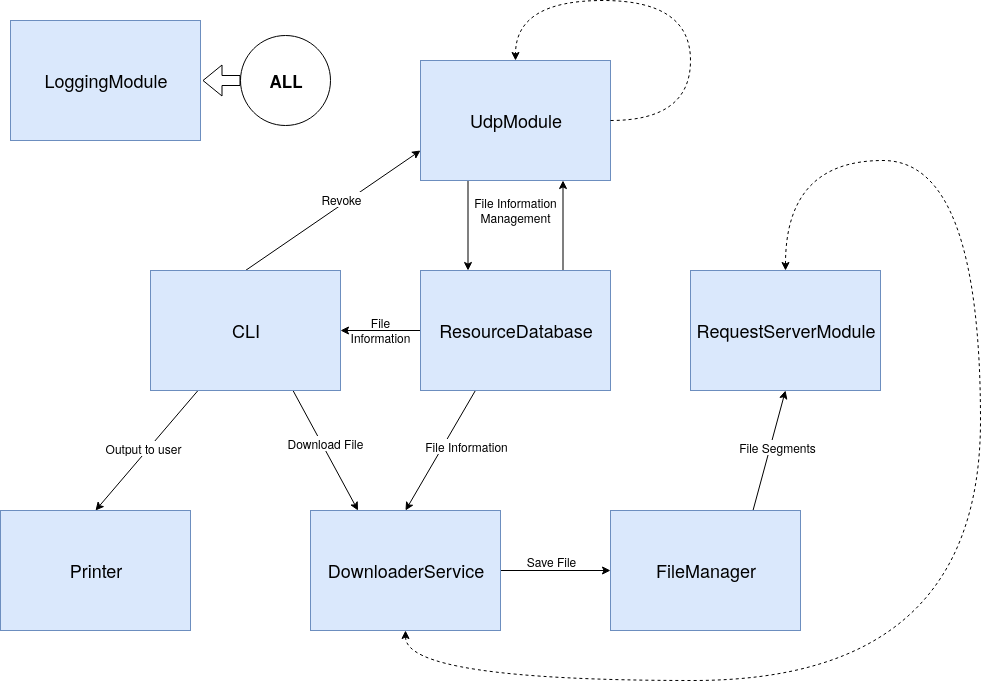
\includegraphics[width=\textwidth]{modules}
\end{centering}

\end{enumerate}
\section{Ważniejsze struktury danych}
\subsection{CompleteResource}
Klasa reprezentująca kompletny zasób, przechowująca zarówno wskaźnik do zbuforowanej zawartości pliku, jak i informacje o nim, takie jak lista hostów będących w jego posiadaniu. Ponadto klasa ta jest przystosowana do pobierania pliku w postaci jedno-kilobajtowych segmentów i do kompletowania ich w różnej kolejności. \\
W momencie pobierania zasobu przez sieć wiele wątków pobiera współbieżnie różne segmenty zasobu. Każdy z wątków ma dostęp do obiektu klasy \textit{CompleteResource}. Klasa ta przechowuje bitsety niosące informacje o tym, które segmenty są aktualnie pobierane, które są już pobrane, a których jeszcze nie pobrano. Wątki pobierające modyfikują te bitsety poprzez odpowiednie metody klasa zapewnia synchronizację dostępu do bitsetów.
\subsection{ResourceDatabase}
\textit{ResourceDatabase} można przybliżyć jako graf dwudzielny którego jedna z klas dwudzielności to hosty a druga pliki posiadane przez odpowiednie hosty.
Szczególnym przypadkiem hosta jest host lokalny czyli komputer na którym działa program.\\
\begin{centering}
	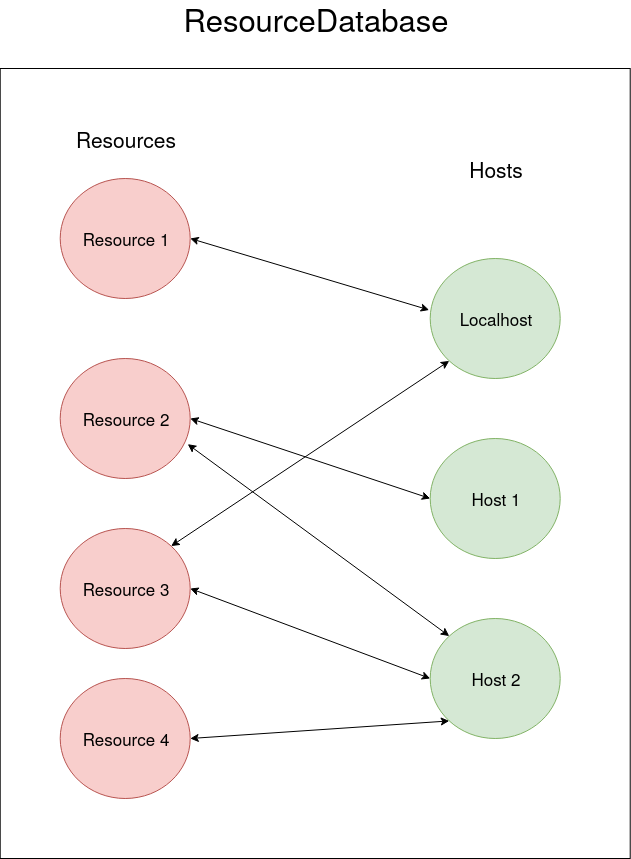
\includegraphics[width=\textwidth]{database}
\end{centering}
\section{Obsługa Sytuacji Wyjatkowych}
\begin{enumerate}
	\item 
	\textit{Opuszczenie przez węzeł sieci :} \\
	po nie otrzymaniu od któregoś z węzłów sieci rozgłoszenia przez kilka okresów rozgłoszeń informacja o posiadaniu przez niego plików jest usuwana z systemu. Ze względu na fakt istnienia weak\_ptr  w kopiach hostów posiadających plik, informacja o jego istnieniu nie jest usuwana z bazy danych
	\item
\textit{	Opóźnione działanie węzła sieci :}\\
	Dla każdego z węzłów prowadzone jest zliczanie prekroczeń ustalonego czasu przy odpowiedziach na zapytania. Po odczekaniu pewnego czasu [ban time] próbujemy ponownie, jesli węzeł znów odpowiada z opóźnieniem nie pobieramy od niego segmentów.
	jeśli wszystkie węzły są opóźnione kończymy pobieranie.
	\item
	\textit{Błąd przy odbiorze danych przez TCP :}\\
	wątek pobierający od danego Hosta zwalnia segment oraz kończy pracę
	\item
\textit{	Gubienie rozgłaszanych pakietów: }\\
	 Udp rozgłasza pakiety fragmentami. Fragmenty są mniejsze niż 2*576 oktetów co oznacza że w przypadku działania w sieci przewodowej ryzyko zgubienia pakiety będzie minimalne [mtu = 1500 oktetów], a w przypadku sieci bezprzewodowej przynajmniej co któryś pakiet dotrze w całości. W przypadku notorycznego gubienia pakietów węzeł będzie niewidoczny dla pozostałych.
	
\end{enumerate}
\section{Testy}
Aplikacja została sprawdzona pod kątek działania w sieci wifi na2 osobnych maszynach
\begin{enumerate}
	\item Sprawdzono poprawność rozgłoszeń, obserwując ruch wiresharkiem.
	\item Sprawdzono poprawność rozgłoszeń w programie.
	\item Sprawdzono działanie unieważnień w programie.
	\item Sprawdzono doświadczalnie na przykładzie kilkumegabajtowego pliku zdolność programu do wypełniania głównego zadania
\end{enumerate}

\part{Dokumentacja kodu źródłowego - \textit{English}}
\chapter{Class Index}
\section{Class List}
Here are the classes, structs, unions and interfaces with brief descriptions\+:\begin{DoxyCompactList}
\item\contentsline{section}{\hyperlink{classSimpleP2P_1_1FileManager}{Simple\+P2\+P\+::\+File\+Manager} \\*Handles read/write to the files on disc }{\pageref{classSimpleP2P_1_1FileManager}}{}
\item\contentsline{section}{\hyperlink{classSimpleP2P_1_1FileRequest}{Simple\+P2\+P\+::\+File\+Request} \\*Carries info about a single file transfer request -\/ resource header and numbers of wanted segments }{\pageref{classSimpleP2P_1_1FileRequest}}{}
\item\contentsline{section}{\hyperlink{classsimpleP2P_1_1Host}{simple\+P2\+P\+::\+Host} \\*Forward declaration }{\pageref{classsimpleP2P_1_1Host}}{}
\item\contentsline{section}{\hyperlink{classsimpleP2P_1_1Logging__Module}{simple\+P2\+P\+::\+Logging\+\_\+\+Module} \\*Class Providing logging support based on text logs }{\pageref{classsimpleP2P_1_1Logging__Module}}{}
\item\contentsline{section}{\hyperlink{classSimpleP2P_1_1RequestServer}{Simple\+P2\+P\+::\+Request\+Server} \\*Asynchronous T\+CP server }{\pageref{classSimpleP2P_1_1RequestServer}}{}
\item\contentsline{section}{\hyperlink{classSimpleP2P_1_1RequestServerModule}{Simple\+P2\+P\+::\+Request\+Server\+Module} \\*Module of the T\+CP server receiving file requests and sending the requested files\textquotesingle{} segments }{\pageref{classSimpleP2P_1_1RequestServerModule}}{}
\item\contentsline{section}{\hyperlink{classSimpleP2P_1_1RequestWorker}{Simple\+P2\+P\+::\+Request\+Worker} \\*T\+CP connection handler, created by the T\+CP server }{\pageref{classSimpleP2P_1_1RequestWorker}}{}
\item\contentsline{section}{\hyperlink{classsimpleP2P_1_1Resource}{simple\+P2\+P\+::\+Resource} \\*Forward declaration }{\pageref{classsimpleP2P_1_1Resource}}{}
\item\contentsline{section}{\hyperlink{classsimpleP2P_1_1Resource__Database}{simple\+P2\+P\+::\+Resource\+\_\+\+Database} \\*Class holding information about files in network and on localhost }{\pageref{classsimpleP2P_1_1Resource__Database}}{}
\item\contentsline{section}{\hyperlink{classsimpleP2P_1_1Udp__Client}{simple\+P2\+P\+::\+Udp\+\_\+\+Client} \\*Class U\+DP Client to handle all outgoing packets }{\pageref{classsimpleP2P_1_1Udp__Client}}{}
\item\contentsline{section}{\hyperlink{classsimpleP2P_1_1Udp__Module}{simple\+P2\+P\+::\+Udp\+\_\+\+Module} \\*Class containing all U\+DP related resources and logic }{\pageref{classsimpleP2P_1_1Udp__Module}}{}
\item\contentsline{section}{\hyperlink{classsimpleP2P_1_1Udp__Server}{simple\+P2\+P\+::\+Udp\+\_\+\+Server} \\*Class U\+DP Server to handle all incoming packets }{\pageref{classsimpleP2P_1_1Udp__Server}}{}
\end{DoxyCompactList}

\chapter{Class Documentation}
\hypertarget{classsimpleP2P_1_1CLI}{}\section{simple\+P2P\+:\+:C\+LI Class Reference}
\label{classsimpleP2P_1_1CLI}\index{simple\+P2\+P\+::\+C\+LI@{simple\+P2\+P\+::\+C\+LI}}
\subsection*{Public Member Functions}
\begin{DoxyCompactItemize}
\item 
\mbox{\Hypertarget{classsimpleP2P_1_1CLI_ad050c491b2185e4230f47ff504f7e0ac}\label{classsimpleP2P_1_1CLI_ad050c491b2185e4230f47ff504f7e0ac}} 
{\bfseries C\+LI} (\hyperlink{classsimpleP2P_1_1Resource__Database}{Resource\+\_\+\+Database} \&res\+\_\+db\+\_\+, \hyperlink{classsimpleP2P_1_1Logging__Module}{Logging\+\_\+\+Module} \&Logger\+\_\+, boost\+::asio\+::io\+\_\+service \&io\+\_\+service\+\_\+, \hyperlink{classsimpleP2P_1_1FileManager}{File\+Manager} \&fm\+\_\+, \hyperlink{classsimpleP2P_1_1Host}{Host} \&localhost\+\_\+, \hyperlink{classsimpleP2P_1_1Printer}{Printer} \&printer\+\_\+)
\item 
\mbox{\Hypertarget{classsimpleP2P_1_1CLI_a66ffb438b7ad05e349f6469bf5574521}\label{classsimpleP2P_1_1CLI_a66ffb438b7ad05e349f6469bf5574521}} 
std\+::thread {\bfseries init} ()
\end{DoxyCompactItemize}


The documentation for this class was generated from the following files\+:\begin{DoxyCompactItemize}
\item 
include/C\+L\+I.\+h\item 
src/C\+L\+I.\+cpp\end{DoxyCompactItemize}

\hypertarget{classsimpleP2P_1_1CLICommand}{}\section{simple\+P2P\+:\+:C\+L\+I\+Command Class Reference}
\label{classsimpleP2P_1_1CLICommand}\index{simple\+P2\+P\+::\+C\+L\+I\+Command@{simple\+P2\+P\+::\+C\+L\+I\+Command}}
\subsection*{Public Member Functions}
\begin{DoxyCompactItemize}
\item 
\mbox{\Hypertarget{classsimpleP2P_1_1CLICommand_a9d983edd720847832774517bb2d74b76}\label{classsimpleP2P_1_1CLICommand_a9d983edd720847832774517bb2d74b76}} 
{\bfseries C\+L\+I\+Command} (std\+::string, std\+::string, std\+::function$<$ Int32(const std\+::string \&)$>$)
\item 
\mbox{\Hypertarget{classsimpleP2P_1_1CLICommand_a664d1534687bb9d11f0d613bca6febd5}\label{classsimpleP2P_1_1CLICommand_a664d1534687bb9d11f0d613bca6febd5}} 
void {\bfseries operator()} (std\+::string) const
\item 
\mbox{\Hypertarget{classsimpleP2P_1_1CLICommand_adad7522128a241e41725e161a63726c6}\label{classsimpleP2P_1_1CLICommand_adad7522128a241e41725e161a63726c6}} 
std\+::string {\bfseries get\+Name} () const
\item 
\mbox{\Hypertarget{classsimpleP2P_1_1CLICommand_a87f9a294e43f062b23639f40b0e5a518}\label{classsimpleP2P_1_1CLICommand_a87f9a294e43f062b23639f40b0e5a518}} 
std\+::string {\bfseries get\+Desc} () const
\end{DoxyCompactItemize}


The documentation for this class was generated from the following files\+:\begin{DoxyCompactItemize}
\item 
include/C\+L\+I\+Command.\+h\item 
src/C\+L\+I\+Command.\+cpp\end{DoxyCompactItemize}

\hypertarget{classsimpleP2P_1_1CompleteResource}{}\section{simple\+P2P\+:\+:Complete\+Resource Class Reference}
\label{classsimpleP2P_1_1CompleteResource}\index{simple\+P2\+P\+::\+Complete\+Resource@{simple\+P2\+P\+::\+Complete\+Resource}}


Class representing a complete resource (resource and full its data)  




{\ttfamily \#include $<$Complete\+Resource.\+h$>$}

\subsection*{Public Member Functions}
\begin{DoxyCompactItemize}
\item 
\hyperlink{classsimpleP2P_1_1CompleteResource_a758df5fa183938450b71d1e36af8fbaf}{Complete\+Resource} (std\+::shared\+\_\+ptr$<$ \hyperlink{classsimpleP2P_1_1Resource}{Resource} $>$ resource\+\_\+c)
\begin{DoxyCompactList}\small\item\em Construct a new Complete \hyperlink{classsimpleP2P_1_1Resource}{Resource} object based on base \hyperlink{classsimpleP2P_1_1Resource}{Resource} object. \end{DoxyCompactList}\item 
Uint8 $\ast$ \hyperlink{classsimpleP2P_1_1CompleteResource_a28c22b852e21d864086440b82822ffa3}{get\+\_\+data} ()
\begin{DoxyCompactList}\small\item\em Get the contents of the file. \end{DoxyCompactList}\item 
std\+::shared\+\_\+ptr$<$ \hyperlink{classsimpleP2P_1_1Resource}{Resource} $>$ \hyperlink{classsimpleP2P_1_1CompleteResource_ac31825cc3bed61d181456430db3878f4}{get\+\_\+resource} () const
\begin{DoxyCompactList}\small\item\em Get the underlaying resource object. \end{DoxyCompactList}\item 
\hyperlink{classsimpleP2P_1_1Segment}{Segment} \hyperlink{classsimpleP2P_1_1CompleteResource_aabe86fbdc8daab23c1df0bc2abb91e7d}{get\+\_\+segment} ()
\begin{DoxyCompactList}\small\item\em Synchronised method returning \hyperlink{classsimpleP2P_1_1Segment}{Segment} object representing the first unbusy and incomplete segment. \end{DoxyCompactList}\item 
void \hyperlink{classsimpleP2P_1_1CompleteResource_a52ddae2486fb593cc315247af38014e7}{set\+\_\+segment} (\hyperlink{classsimpleP2P_1_1Segment}{Segment} \&segment)
\begin{DoxyCompactList}\small\item\em Synchronised method marking the given segment as completed. \end{DoxyCompactList}\item 
bool \hyperlink{classsimpleP2P_1_1CompleteResource_aaa20fce1d1d3fbd3f616debaedcaf7a3}{is\+\_\+completed} ()
\begin{DoxyCompactList}\small\item\em Synchronised method returning true if all segments have been downloaded, false otherwise. \end{DoxyCompactList}\item 
void \hyperlink{classsimpleP2P_1_1CompleteResource_af2dd5d30d807b11ecdad7feaf488df89}{unset\+\_\+busy} (Segment\+Id id)
\begin{DoxyCompactList}\small\item\em Synchronised method unmarking busy segment and notifying one of waithing worker threads. \end{DoxyCompactList}\end{DoxyCompactItemize}


\subsection{Detailed Description}
Class representing a complete resource (resource and full its data) 



\subsection{Constructor \& Destructor Documentation}
\mbox{\Hypertarget{classsimpleP2P_1_1CompleteResource_a758df5fa183938450b71d1e36af8fbaf}\label{classsimpleP2P_1_1CompleteResource_a758df5fa183938450b71d1e36af8fbaf}} 
\index{simple\+P2\+P\+::\+Complete\+Resource@{simple\+P2\+P\+::\+Complete\+Resource}!Complete\+Resource@{Complete\+Resource}}
\index{Complete\+Resource@{Complete\+Resource}!simple\+P2\+P\+::\+Complete\+Resource@{simple\+P2\+P\+::\+Complete\+Resource}}
\subsubsection{\texorpdfstring{Complete\+Resource()}{CompleteResource()}}
{\footnotesize\ttfamily simple\+P2\+P\+::\+Complete\+Resource\+::\+Complete\+Resource (\begin{DoxyParamCaption}\item[{std\+::shared\+\_\+ptr$<$ \hyperlink{classsimpleP2P_1_1Resource}{Resource} $>$}]{resource\+\_\+c }\end{DoxyParamCaption})}



Construct a new Complete \hyperlink{classsimpleP2P_1_1Resource}{Resource} object based on base \hyperlink{classsimpleP2P_1_1Resource}{Resource} object. 


\begin{DoxyParams}{Parameters}
{\em resource\+\_\+c} & base resource object \\
\hline
\end{DoxyParams}


\subsection{Member Function Documentation}
\mbox{\Hypertarget{classsimpleP2P_1_1CompleteResource_a28c22b852e21d864086440b82822ffa3}\label{classsimpleP2P_1_1CompleteResource_a28c22b852e21d864086440b82822ffa3}} 
\index{simple\+P2\+P\+::\+Complete\+Resource@{simple\+P2\+P\+::\+Complete\+Resource}!get\+\_\+data@{get\+\_\+data}}
\index{get\+\_\+data@{get\+\_\+data}!simple\+P2\+P\+::\+Complete\+Resource@{simple\+P2\+P\+::\+Complete\+Resource}}
\subsubsection{\texorpdfstring{get\+\_\+data()}{get\_data()}}
{\footnotesize\ttfamily Uint8 $\ast$ simple\+P2\+P\+::\+Complete\+Resource\+::get\+\_\+data (\begin{DoxyParamCaption}{ }\end{DoxyParamCaption})}



Get the contents of the file. 

\begin{DoxyReturn}{Returns}
Uint8$\ast$ 
\end{DoxyReturn}
\mbox{\Hypertarget{classsimpleP2P_1_1CompleteResource_ac31825cc3bed61d181456430db3878f4}\label{classsimpleP2P_1_1CompleteResource_ac31825cc3bed61d181456430db3878f4}} 
\index{simple\+P2\+P\+::\+Complete\+Resource@{simple\+P2\+P\+::\+Complete\+Resource}!get\+\_\+resource@{get\+\_\+resource}}
\index{get\+\_\+resource@{get\+\_\+resource}!simple\+P2\+P\+::\+Complete\+Resource@{simple\+P2\+P\+::\+Complete\+Resource}}
\subsubsection{\texorpdfstring{get\+\_\+resource()}{get\_resource()}}
{\footnotesize\ttfamily std\+::shared\+\_\+ptr$<$ \hyperlink{classsimpleP2P_1_1Resource}{Resource} $>$ simple\+P2\+P\+::\+Complete\+Resource\+::get\+\_\+resource (\begin{DoxyParamCaption}{ }\end{DoxyParamCaption}) const}



Get the underlaying resource object. 

\begin{DoxyReturn}{Returns}
std\+::shared\+\_\+ptr$<$\+Resource$>$ 
\end{DoxyReturn}
\mbox{\Hypertarget{classsimpleP2P_1_1CompleteResource_aabe86fbdc8daab23c1df0bc2abb91e7d}\label{classsimpleP2P_1_1CompleteResource_aabe86fbdc8daab23c1df0bc2abb91e7d}} 
\index{simple\+P2\+P\+::\+Complete\+Resource@{simple\+P2\+P\+::\+Complete\+Resource}!get\+\_\+segment@{get\+\_\+segment}}
\index{get\+\_\+segment@{get\+\_\+segment}!simple\+P2\+P\+::\+Complete\+Resource@{simple\+P2\+P\+::\+Complete\+Resource}}
\subsubsection{\texorpdfstring{get\+\_\+segment()}{get\_segment()}}
{\footnotesize\ttfamily \hyperlink{classsimpleP2P_1_1Segment}{Segment} simple\+P2\+P\+::\+Complete\+Resource\+::get\+\_\+segment (\begin{DoxyParamCaption}{ }\end{DoxyParamCaption})}



Synchronised method returning \hyperlink{classsimpleP2P_1_1Segment}{Segment} object representing the first unbusy and incomplete segment. 

If resource downlaoding has been completed, special \hyperlink{classsimpleP2P_1_1Segment}{Segment} object with id set to N\+O\+\_\+\+S\+E\+G\+M\+E\+N\+T\+\_\+\+ID is returned. If there is no appropriate segment found and downloading is not completed, method suspends calling worker thread pending some segment release.

\begin{DoxyReturn}{Returns}
\hyperlink{classsimpleP2P_1_1Segment}{Segment} 
\end{DoxyReturn}
\mbox{\Hypertarget{classsimpleP2P_1_1CompleteResource_aaa20fce1d1d3fbd3f616debaedcaf7a3}\label{classsimpleP2P_1_1CompleteResource_aaa20fce1d1d3fbd3f616debaedcaf7a3}} 
\index{simple\+P2\+P\+::\+Complete\+Resource@{simple\+P2\+P\+::\+Complete\+Resource}!is\+\_\+completed@{is\+\_\+completed}}
\index{is\+\_\+completed@{is\+\_\+completed}!simple\+P2\+P\+::\+Complete\+Resource@{simple\+P2\+P\+::\+Complete\+Resource}}
\subsubsection{\texorpdfstring{is\+\_\+completed()}{is\_completed()}}
{\footnotesize\ttfamily bool simple\+P2\+P\+::\+Complete\+Resource\+::is\+\_\+completed (\begin{DoxyParamCaption}{ }\end{DoxyParamCaption})}



Synchronised method returning true if all segments have been downloaded, false otherwise. 

\begin{DoxyReturn}{Returns}
true if downloading is completed 

false otherwise 
\end{DoxyReturn}
\mbox{\Hypertarget{classsimpleP2P_1_1CompleteResource_a52ddae2486fb593cc315247af38014e7}\label{classsimpleP2P_1_1CompleteResource_a52ddae2486fb593cc315247af38014e7}} 
\index{simple\+P2\+P\+::\+Complete\+Resource@{simple\+P2\+P\+::\+Complete\+Resource}!set\+\_\+segment@{set\+\_\+segment}}
\index{set\+\_\+segment@{set\+\_\+segment}!simple\+P2\+P\+::\+Complete\+Resource@{simple\+P2\+P\+::\+Complete\+Resource}}
\subsubsection{\texorpdfstring{set\+\_\+segment()}{set\_segment()}}
{\footnotesize\ttfamily void simple\+P2\+P\+::\+Complete\+Resource\+::set\+\_\+segment (\begin{DoxyParamCaption}\item[{\hyperlink{classsimpleP2P_1_1Segment}{Segment} \&}]{segment }\end{DoxyParamCaption})}



Synchronised method marking the given segment as completed. 

If all segments have been downloaded, method notifies all waiting worker threads so that they can join.


\begin{DoxyParams}{Parameters}
{\em segment} & \\
\hline
\end{DoxyParams}
\mbox{\Hypertarget{classsimpleP2P_1_1CompleteResource_af2dd5d30d807b11ecdad7feaf488df89}\label{classsimpleP2P_1_1CompleteResource_af2dd5d30d807b11ecdad7feaf488df89}} 
\index{simple\+P2\+P\+::\+Complete\+Resource@{simple\+P2\+P\+::\+Complete\+Resource}!unset\+\_\+busy@{unset\+\_\+busy}}
\index{unset\+\_\+busy@{unset\+\_\+busy}!simple\+P2\+P\+::\+Complete\+Resource@{simple\+P2\+P\+::\+Complete\+Resource}}
\subsubsection{\texorpdfstring{unset\+\_\+busy()}{unset\_busy()}}
{\footnotesize\ttfamily void simple\+P2\+P\+::\+Complete\+Resource\+::unset\+\_\+busy (\begin{DoxyParamCaption}\item[{Segment\+Id}]{id }\end{DoxyParamCaption})}



Synchronised method unmarking busy segment and notifying one of waithing worker threads. 


\begin{DoxyParams}{Parameters}
{\em id} & \\
\hline
\end{DoxyParams}


The documentation for this class was generated from the following files\+:\begin{DoxyCompactItemize}
\item 
include/Complete\+Resource.\+h\item 
src/Complete\+Resource.\+cpp\end{DoxyCompactItemize}

\hypertarget{classsimpleP2P_1_1DownloadService}{}\section{simple\+P2P\+:\+:Download\+Service Class Reference}
\label{classsimpleP2P_1_1DownloadService}\index{simple\+P2\+P\+::\+Download\+Service@{simple\+P2\+P\+::\+Download\+Service}}


Used to download resource.  




{\ttfamily \#include $<$Download\+Service.\+h$>$}

\subsection*{Public Member Functions}
\begin{DoxyCompactItemize}
\item 
\hyperlink{classsimpleP2P_1_1DownloadService_a3d0394fd9f3c7a954ad3dbe6249fbf42}{Download\+Service} (\hyperlink{classsimpleP2P_1_1LoggingModule}{Logging\+Module} \&logging\+\_\+module\+\_\+c, boost\+::asio\+::io\+\_\+service \&io\+\_\+service\+\_\+c, \hyperlink{classsimpleP2P_1_1FileManager}{File\+Manager} \&file\+\_\+manager\+\_\+c, \hyperlink{classsimpleP2P_1_1ResourceDatabase}{Resource\+Database} \&resource\+\_\+database\+\_\+c, std\+::shared\+\_\+ptr$<$ \hyperlink{classsimpleP2P_1_1Resource}{Resource} $>$ resource\+\_\+c)
\begin{DoxyCompactList}\small\item\em Construct a new Download Service object. \end{DoxyCompactList}\item 
\mbox{\Hypertarget{classsimpleP2P_1_1DownloadService_ab16e0deab0bba9b03a251a3ff5af114c}\label{classsimpleP2P_1_1DownloadService_ab16e0deab0bba9b03a251a3ff5af114c}} 
void \hyperlink{classsimpleP2P_1_1DownloadService_ab16e0deab0bba9b03a251a3ff5af114c}{init} ()
\begin{DoxyCompactList}\small\item\em Method initiating downloading in the current thread. \end{DoxyCompactList}\item 
std\+::thread \hyperlink{classsimpleP2P_1_1DownloadService_a420979e6932be2f09bcc2b34e7ac8b7a}{init\+\_\+thread} ()
\begin{DoxyCompactList}\small\item\em Method initiating downloading in a new thread. \end{DoxyCompactList}\end{DoxyCompactItemize}


\subsection{Detailed Description}
Used to download resource. 

\subsection{Constructor \& Destructor Documentation}
\mbox{\Hypertarget{classsimpleP2P_1_1DownloadService_a3d0394fd9f3c7a954ad3dbe6249fbf42}\label{classsimpleP2P_1_1DownloadService_a3d0394fd9f3c7a954ad3dbe6249fbf42}} 
\index{simple\+P2\+P\+::\+Download\+Service@{simple\+P2\+P\+::\+Download\+Service}!Download\+Service@{Download\+Service}}
\index{Download\+Service@{Download\+Service}!simple\+P2\+P\+::\+Download\+Service@{simple\+P2\+P\+::\+Download\+Service}}
\subsubsection{\texorpdfstring{Download\+Service()}{DownloadService()}}
{\footnotesize\ttfamily simple\+P2\+P\+::\+Download\+Service\+::\+Download\+Service (\begin{DoxyParamCaption}\item[{\hyperlink{classsimpleP2P_1_1LoggingModule}{Logging\+Module} \&}]{logging\+\_\+module\+\_\+c,  }\item[{boost\+::asio\+::io\+\_\+service \&}]{io\+\_\+service\+\_\+c,  }\item[{\hyperlink{classsimpleP2P_1_1FileManager}{File\+Manager} \&}]{file\+\_\+manager\+\_\+c,  }\item[{\hyperlink{classsimpleP2P_1_1ResourceDatabase}{Resource\+Database} \&}]{resource\+\_\+database\+\_\+c,  }\item[{std\+::shared\+\_\+ptr$<$ \hyperlink{classsimpleP2P_1_1Resource}{Resource} $>$}]{resource\+\_\+c }\end{DoxyParamCaption})}



Construct a new Download Service object. 


\begin{DoxyParams}{Parameters}
{\em logging\+\_\+module\+\_\+c} & \\
\hline
{\em io\+\_\+service\+\_\+c} & \\
\hline
{\em file\+\_\+manager\+\_\+c} & \\
\hline
{\em resource\+\_\+database\+\_\+c} & \\
\hline
{\em resource\+\_\+c} & \\
\hline
\end{DoxyParams}


\subsection{Member Function Documentation}
\mbox{\Hypertarget{classsimpleP2P_1_1DownloadService_a420979e6932be2f09bcc2b34e7ac8b7a}\label{classsimpleP2P_1_1DownloadService_a420979e6932be2f09bcc2b34e7ac8b7a}} 
\index{simple\+P2\+P\+::\+Download\+Service@{simple\+P2\+P\+::\+Download\+Service}!init\+\_\+thread@{init\+\_\+thread}}
\index{init\+\_\+thread@{init\+\_\+thread}!simple\+P2\+P\+::\+Download\+Service@{simple\+P2\+P\+::\+Download\+Service}}
\subsubsection{\texorpdfstring{init\+\_\+thread()}{init\_thread()}}
{\footnotesize\ttfamily std\+::thread simple\+P2\+P\+::\+Download\+Service\+::init\+\_\+thread (\begin{DoxyParamCaption}{ }\end{DoxyParamCaption})}



Method initiating downloading in a new thread. 

\begin{DoxyReturn}{Returns}
std\+::thread 
\end{DoxyReturn}


The documentation for this class was generated from the following files\+:\begin{DoxyCompactItemize}
\item 
include/Download\+Service.\+h\item 
src/Download\+Service.\+cpp\end{DoxyCompactItemize}

\hypertarget{classsimpleP2P_1_1DownloadWorker}{}\section{simple\+P2P\+:\+:Download\+Worker Class Reference}
\label{classsimpleP2P_1_1DownloadWorker}\index{simple\+P2\+P\+::\+Download\+Worker@{simple\+P2\+P\+::\+Download\+Worker}}


Class used to download resource segments from one host.  




{\ttfamily \#include $<$Download\+Worker.\+h$>$}

\subsection*{Public Member Functions}
\begin{DoxyCompactItemize}
\item 
\hyperlink{classsimpleP2P_1_1DownloadWorker_a2861145541d88a86bf3b082e5272d1d8}{Download\+Worker} (\hyperlink{classsimpleP2P_1_1LoggingModule}{Logging\+Module} \&logging\+\_\+module\+\_\+c, boost\+::asio\+::io\+\_\+service \&io\+\_\+service\+\_\+c, std\+::shared\+\_\+ptr$<$ \hyperlink{classsimpleP2P_1_1Host}{Host} $>$ host\+\_\+c, std\+::shared\+\_\+ptr$<$ \hyperlink{classsimpleP2P_1_1CompleteResource}{Complete\+Resource} $>$ complete\+\_\+resource\+\_\+c)
\begin{DoxyCompactList}\small\item\em Construct a new Download Worker object. \end{DoxyCompactList}\item 
std\+::thread \hyperlink{classsimpleP2P_1_1DownloadWorker_aedf77c7a4944beaee84494c83512551b}{init} ()
\begin{DoxyCompactList}\small\item\em Method initiating connection to host and downloading resource segments in a new thread. \end{DoxyCompactList}\item 
void \hyperlink{classsimpleP2P_1_1DownloadWorker_a03f21eb4f4d1a1e3e87f983ff5e389f7}{check\+\_\+timeout} ()
\begin{DoxyCompactList}\small\item\em Method checking worker timeout and taking appropriate actions if it exeeds\+: \end{DoxyCompactList}\item 
void \hyperlink{classsimpleP2P_1_1DownloadWorker_ae975a4408ee3e8f85c0a067732dd44f0}{close} ()
\begin{DoxyCompactList}\small\item\em ++ \end{DoxyCompactList}\item 
\mbox{\Hypertarget{classsimpleP2P_1_1DownloadWorker_a5e46b7b54882ef35bfaf48b51573a96e}\label{classsimpleP2P_1_1DownloadWorker_a5e46b7b54882ef35bfaf48b51573a96e}} 
bool \hyperlink{classsimpleP2P_1_1DownloadWorker_a5e46b7b54882ef35bfaf48b51573a96e}{is\+\_\+closed} ()
\begin{DoxyCompactList}\small\item\em Synchronised method checking if worker is closed. \end{DoxyCompactList}\item 
bool \hyperlink{classsimpleP2P_1_1DownloadWorker_a73743cf5fe1e579bc7cf0e5acb504450}{is\+\_\+unavailable} ()
\begin{DoxyCompactList}\small\item\em Synchronised method checking if worker is available (not closed and associated host not retarded) \end{DoxyCompactList}\end{DoxyCompactItemize}


\subsection{Detailed Description}
Class used to download resource segments from one host. 

\subsection{Constructor \& Destructor Documentation}
\mbox{\Hypertarget{classsimpleP2P_1_1DownloadWorker_a2861145541d88a86bf3b082e5272d1d8}\label{classsimpleP2P_1_1DownloadWorker_a2861145541d88a86bf3b082e5272d1d8}} 
\index{simple\+P2\+P\+::\+Download\+Worker@{simple\+P2\+P\+::\+Download\+Worker}!Download\+Worker@{Download\+Worker}}
\index{Download\+Worker@{Download\+Worker}!simple\+P2\+P\+::\+Download\+Worker@{simple\+P2\+P\+::\+Download\+Worker}}
\subsubsection{\texorpdfstring{Download\+Worker()}{DownloadWorker()}}
{\footnotesize\ttfamily simple\+P2\+P\+::\+Download\+Worker\+::\+Download\+Worker (\begin{DoxyParamCaption}\item[{\hyperlink{classsimpleP2P_1_1LoggingModule}{Logging\+Module} \&}]{logging\+\_\+module\+\_\+c,  }\item[{boost\+::asio\+::io\+\_\+service \&}]{io\+\_\+service\+\_\+c,  }\item[{std\+::shared\+\_\+ptr$<$ \hyperlink{classsimpleP2P_1_1Host}{Host} $>$}]{host\+\_\+c,  }\item[{std\+::shared\+\_\+ptr$<$ \hyperlink{classsimpleP2P_1_1CompleteResource}{Complete\+Resource} $>$}]{complete\+\_\+resource\+\_\+c }\end{DoxyParamCaption})}



Construct a new Download Worker object. 


\begin{DoxyParams}{Parameters}
{\em logging\+\_\+module\+\_\+c} & \\
\hline
{\em io\+\_\+service\+\_\+c} & \\
\hline
{\em host\+\_\+c} & \\
\hline
{\em complete\+\_\+resource\+\_\+c} & \\
\hline
\end{DoxyParams}


\subsection{Member Function Documentation}
\mbox{\Hypertarget{classsimpleP2P_1_1DownloadWorker_a03f21eb4f4d1a1e3e87f983ff5e389f7}\label{classsimpleP2P_1_1DownloadWorker_a03f21eb4f4d1a1e3e87f983ff5e389f7}} 
\index{simple\+P2\+P\+::\+Download\+Worker@{simple\+P2\+P\+::\+Download\+Worker}!check\+\_\+timeout@{check\+\_\+timeout}}
\index{check\+\_\+timeout@{check\+\_\+timeout}!simple\+P2\+P\+::\+Download\+Worker@{simple\+P2\+P\+::\+Download\+Worker}}
\subsubsection{\texorpdfstring{check\+\_\+timeout()}{check\_timeout()}}
{\footnotesize\ttfamily void simple\+P2\+P\+::\+Download\+Worker\+::check\+\_\+timeout (\begin{DoxyParamCaption}{ }\end{DoxyParamCaption})}



Method checking worker timeout and taking appropriate actions if it exeeds\+: 


\begin{DoxyItemize}
\item the host timeout counter is increased, what may cause banning host for certain time,
\item currently downloaded segment is marked as unbusy and may be downloaded by another worker. 
\end{DoxyItemize}\mbox{\Hypertarget{classsimpleP2P_1_1DownloadWorker_ae975a4408ee3e8f85c0a067732dd44f0}\label{classsimpleP2P_1_1DownloadWorker_ae975a4408ee3e8f85c0a067732dd44f0}} 
\index{simple\+P2\+P\+::\+Download\+Worker@{simple\+P2\+P\+::\+Download\+Worker}!close@{close}}
\index{close@{close}!simple\+P2\+P\+::\+Download\+Worker@{simple\+P2\+P\+::\+Download\+Worker}}
\subsubsection{\texorpdfstring{close()}{close()}}
{\footnotesize\ttfamily void simple\+P2\+P\+::\+Download\+Worker\+::close (\begin{DoxyParamCaption}{ }\end{DoxyParamCaption})}



++ 

Synchronised method closing worker politely. \mbox{\Hypertarget{classsimpleP2P_1_1DownloadWorker_aedf77c7a4944beaee84494c83512551b}\label{classsimpleP2P_1_1DownloadWorker_aedf77c7a4944beaee84494c83512551b}} 
\index{simple\+P2\+P\+::\+Download\+Worker@{simple\+P2\+P\+::\+Download\+Worker}!init@{init}}
\index{init@{init}!simple\+P2\+P\+::\+Download\+Worker@{simple\+P2\+P\+::\+Download\+Worker}}
\subsubsection{\texorpdfstring{init()}{init()}}
{\footnotesize\ttfamily std\+::thread simple\+P2\+P\+::\+Download\+Worker\+::init (\begin{DoxyParamCaption}{ }\end{DoxyParamCaption})}



Method initiating connection to host and downloading resource segments in a new thread. 

\begin{DoxyReturn}{Returns}
std\+::thread 
\end{DoxyReturn}
\mbox{\Hypertarget{classsimpleP2P_1_1DownloadWorker_a73743cf5fe1e579bc7cf0e5acb504450}\label{classsimpleP2P_1_1DownloadWorker_a73743cf5fe1e579bc7cf0e5acb504450}} 
\index{simple\+P2\+P\+::\+Download\+Worker@{simple\+P2\+P\+::\+Download\+Worker}!is\+\_\+unavailable@{is\+\_\+unavailable}}
\index{is\+\_\+unavailable@{is\+\_\+unavailable}!simple\+P2\+P\+::\+Download\+Worker@{simple\+P2\+P\+::\+Download\+Worker}}
\subsubsection{\texorpdfstring{is\+\_\+unavailable()}{is\_unavailable()}}
{\footnotesize\ttfamily bool simple\+P2\+P\+::\+Download\+Worker\+::is\+\_\+unavailable (\begin{DoxyParamCaption}{ }\end{DoxyParamCaption})}



Synchronised method checking if worker is available (not closed and associated host not retarded) 

\begin{DoxyReturn}{Returns}
true 

false 
\end{DoxyReturn}


The documentation for this class was generated from the following files\+:\begin{DoxyCompactItemize}
\item 
include/Download\+Worker.\+h\item 
src/Download\+Worker.\+cpp\end{DoxyCompactItemize}

\hypertarget{classsimpleP2P_1_1FileManager}{}\section{simple\+P2P\+:\+:File\+Manager Class Reference}
\label{classsimpleP2P_1_1FileManager}\index{simple\+P2\+P\+::\+File\+Manager@{simple\+P2\+P\+::\+File\+Manager}}


Handles read/write to the files on disc.  




{\ttfamily \#include $<$File\+Manager.\+h$>$}

\subsection*{Public Member Functions}
\begin{DoxyCompactItemize}
\item 
\mbox{\Hypertarget{classsimpleP2P_1_1FileManager_a335188a96b1d257ed0ecdaf76befec95}\label{classsimpleP2P_1_1FileManager_a335188a96b1d257ed0ecdaf76befec95}} 
{\bfseries File\+Manager} (\hyperlink{classsimpleP2P_1_1LoggingModule}{Logging\+Module} \&lm)
\item 
bool \hyperlink{classsimpleP2P_1_1FileManager_ae6d78d28f40cc7fabe16de7a124a38be}{get\+\_\+segment} (const std\+::string file\+\_\+name, const Uint16 segment, Uint8 $\ast$result, const std\+::size\+\_\+t requested\+\_\+segment\+\_\+size)
\begin{DoxyCompactList}\small\item\em Buffers the specificated segment of the specificated file in the char array. \end{DoxyCompactList}\item 
void \hyperlink{classsimpleP2P_1_1FileManager_a120fec780f9a6bf350ffbac731376213}{store\+\_\+resource} (std\+::shared\+\_\+ptr$<$ \hyperlink{classsimpleP2P_1_1CompleteResource}{Complete\+Resource} $>$ complete\+\_\+resource)
\begin{DoxyCompactList}\small\item\em Stores the file contents in the physical file on disc. \end{DoxyCompactList}\item 
bool \hyperlink{classsimpleP2P_1_1FileManager_ad20db5b0d3c3eea9f22ddef7b28c3348}{read\+\_\+lock} (const std\+::string file\+\_\+name)
\begin{DoxyCompactList}\small\item\em Closes the file and unlocks it for writing. \end{DoxyCompactList}\item 
void \hyperlink{classsimpleP2P_1_1FileManager_a5152eb630ec61c6465f3302934696c12}{read\+\_\+unlock} (const std\+::string file\+\_\+name)
\begin{DoxyCompactList}\small\item\em Closes a file which was opened for reading and enables other threads to write to it. \end{DoxyCompactList}\end{DoxyCompactItemize}


\subsection{Detailed Description}
Handles read/write to the files on disc. 

An A\+PI which provides\+:
\begin{DoxyItemize}
\item buffering contents of a requested segment of a specificated local file,
\item storing a complete, downloaded file physically on the local disc. Ensures synchronization of those operations. 
\end{DoxyItemize}

\subsection{Member Function Documentation}
\mbox{\Hypertarget{classsimpleP2P_1_1FileManager_ae6d78d28f40cc7fabe16de7a124a38be}\label{classsimpleP2P_1_1FileManager_ae6d78d28f40cc7fabe16de7a124a38be}} 
\index{simple\+P2\+P\+::\+File\+Manager@{simple\+P2\+P\+::\+File\+Manager}!get\+\_\+segment@{get\+\_\+segment}}
\index{get\+\_\+segment@{get\+\_\+segment}!simple\+P2\+P\+::\+File\+Manager@{simple\+P2\+P\+::\+File\+Manager}}
\subsubsection{\texorpdfstring{get\+\_\+segment()}{get\_segment()}}
{\footnotesize\ttfamily bool simple\+P2\+P\+::\+File\+Manager\+::get\+\_\+segment (\begin{DoxyParamCaption}\item[{const std\+::string}]{file\+\_\+name,  }\item[{const Uint16}]{segment,  }\item[{Uint8 $\ast$}]{result,  }\item[{const std\+::size\+\_\+t}]{requested\+\_\+segment\+\_\+size }\end{DoxyParamCaption})}



Buffers the specificated segment of the specificated file in the char array. 

\begin{DoxyWarning}{Warning}
Calling this function M\+U\+ST be preceded by a successful call to \hyperlink{classsimpleP2P_1_1FileManager_ad20db5b0d3c3eea9f22ddef7b28c3348}{read\+\_\+lock()} on the file specified in resource\+\_\+header equal to the one carried by the Segment\+Request.
\end{DoxyWarning}

\begin{DoxyParams}{Parameters}
{\em request} & Specifies file and its segment to buffer. \\
\hline
{\em result} & The array to buffer the segment in. Its size must be greater or equal to the 3rd parameter! \\
\hline
{\em requested\+\_\+segment\+\_\+size} & Size of the segment to buffer. \\
\hline
\end{DoxyParams}
\begin{DoxyReturn}{Returns}
If the segment has been buffered successfully. 
\end{DoxyReturn}
\mbox{\Hypertarget{classsimpleP2P_1_1FileManager_ad20db5b0d3c3eea9f22ddef7b28c3348}\label{classsimpleP2P_1_1FileManager_ad20db5b0d3c3eea9f22ddef7b28c3348}} 
\index{simple\+P2\+P\+::\+File\+Manager@{simple\+P2\+P\+::\+File\+Manager}!read\+\_\+lock@{read\+\_\+lock}}
\index{read\+\_\+lock@{read\+\_\+lock}!simple\+P2\+P\+::\+File\+Manager@{simple\+P2\+P\+::\+File\+Manager}}
\subsubsection{\texorpdfstring{read\+\_\+lock()}{read\_lock()}}
{\footnotesize\ttfamily bool simple\+P2\+P\+::\+File\+Manager\+::read\+\_\+lock (\begin{DoxyParamCaption}\item[{const std\+::string}]{file\+\_\+name }\end{DoxyParamCaption})}



Closes the file and unlocks it for writing. 


\begin{DoxyParams}{Parameters}
{\em resource\+\_\+header} & The file to be closed and unlocked. Opens a file for reading and prevents other threads from overwriting it until it\textquotesingle{}s closed.\\
\hline
{\em resource\+\_\+header} & The file to be opened and read-\/locked. \\
\hline
\end{DoxyParams}
\begin{DoxyReturn}{Returns}
If the file has been opened successfully. 
\end{DoxyReturn}
\mbox{\Hypertarget{classsimpleP2P_1_1FileManager_a5152eb630ec61c6465f3302934696c12}\label{classsimpleP2P_1_1FileManager_a5152eb630ec61c6465f3302934696c12}} 
\index{simple\+P2\+P\+::\+File\+Manager@{simple\+P2\+P\+::\+File\+Manager}!read\+\_\+unlock@{read\+\_\+unlock}}
\index{read\+\_\+unlock@{read\+\_\+unlock}!simple\+P2\+P\+::\+File\+Manager@{simple\+P2\+P\+::\+File\+Manager}}
\subsubsection{\texorpdfstring{read\+\_\+unlock()}{read\_unlock()}}
{\footnotesize\ttfamily void simple\+P2\+P\+::\+File\+Manager\+::read\+\_\+unlock (\begin{DoxyParamCaption}\item[{const std\+::string}]{file\+\_\+name }\end{DoxyParamCaption})}



Closes a file which was opened for reading and enables other threads to write to it. 

\begin{DoxyWarning}{Warning}
This function M\+U\+ST be called after the reading has completed, so that the file can be overwritten in future.
\end{DoxyWarning}

\begin{DoxyParams}{Parameters}
{\em } & \\
\hline
\end{DoxyParams}
\mbox{\Hypertarget{classsimpleP2P_1_1FileManager_a120fec780f9a6bf350ffbac731376213}\label{classsimpleP2P_1_1FileManager_a120fec780f9a6bf350ffbac731376213}} 
\index{simple\+P2\+P\+::\+File\+Manager@{simple\+P2\+P\+::\+File\+Manager}!store\+\_\+resource@{store\+\_\+resource}}
\index{store\+\_\+resource@{store\+\_\+resource}!simple\+P2\+P\+::\+File\+Manager@{simple\+P2\+P\+::\+File\+Manager}}
\subsubsection{\texorpdfstring{store\+\_\+resource()}{store\_resource()}}
{\footnotesize\ttfamily void simple\+P2\+P\+::\+File\+Manager\+::store\+\_\+resource (\begin{DoxyParamCaption}\item[{std\+::shared\+\_\+ptr$<$ \hyperlink{classsimpleP2P_1_1CompleteResource}{Complete\+Resource} $>$}]{complete\+\_\+resource }\end{DoxyParamCaption})}



Stores the file contents in the physical file on disc. 


\begin{DoxyParams}{Parameters}
{\em resource} & File to store on the disc. The data will not be interpreted, so make sure it\textquotesingle{}s complete and ready to store. \\
\hline
\end{DoxyParams}


The documentation for this class was generated from the following files\+:\begin{DoxyCompactItemize}
\item 
include/File\+Manager.\+h\item 
src/File\+Manager.\+cpp\end{DoxyCompactItemize}

\hypertarget{classsimpleP2P_1_1Host}{}\subsection{simple\+P2P\+:\+:Host Class Reference}
\label{classsimpleP2P_1_1Host}\index{simple\+P2\+P\+::\+Host@{simple\+P2\+P\+::\+Host}}


Forward declaration.  




{\ttfamily \#include $<$host.\+h$>$}

\subsubsection*{Public Member Functions}
\begin{DoxyCompactItemize}
\item 
\hyperlink{classsimpleP2P_1_1Host_abbe0b5c51195b8cf2019d791ace5a5c7}{Host} (boost\+::asio\+::ip\+::address ip)
\begin{DoxyCompactList}\small\item\em Constructor. \end{DoxyCompactList}\item 
bool \hyperlink{classsimpleP2P_1_1Host_a5d4b48eaf05f5353816aae78cbd29c64}{has\+\_\+resource} (\hyperlink{classsimpleP2P_1_1Resource}{Resource} res)
\begin{DoxyCompactList}\small\item\em Determines if host has resource. \end{DoxyCompactList}\item 
bool \hyperlink{classsimpleP2P_1_1Host_aadac09c6ab516f62e5eebe28dd584626}{operator==} (const \hyperlink{classsimpleP2P_1_1Host}{Host} \&other) const
\begin{DoxyCompactList}\small\item\em Operator == checks host\+\_\+ip for equality. \end{DoxyCompactList}\item 
bool \hyperlink{classsimpleP2P_1_1Host_a13516e95bf59bb8dd6eea8940f8bb677}{operator!=} (const \hyperlink{classsimpleP2P_1_1Host}{Host} \&other) const
\begin{DoxyCompactList}\small\item\em Operator != checks host\+\_\+ip for equality. \end{DoxyCompactList}\end{DoxyCompactItemize}
\subsubsection*{Friends}
\begin{DoxyCompactItemize}
\item 
\mbox{\Hypertarget{classsimpleP2P_1_1Host_a8d5b8c31f7b51293954816c91b76cabd}\label{classsimpleP2P_1_1Host_a8d5b8c31f7b51293954816c91b76cabd}} 
class \hyperlink{classsimpleP2P_1_1Host_a8d5b8c31f7b51293954816c91b76cabd}{Resource\+\_\+\+Database}
\begin{DoxyCompactList}\small\item\em friendship to manage \hyperlink{classsimpleP2P_1_1Host}{Host}\textquotesingle{}s Resources timeouts etc \end{DoxyCompactList}\end{DoxyCompactItemize}


\subsubsection{Detailed Description}
Forward declaration. 

Class contains node information and points to files it possess 

\subsubsection{Constructor \& Destructor Documentation}
\mbox{\Hypertarget{classsimpleP2P_1_1Host_abbe0b5c51195b8cf2019d791ace5a5c7}\label{classsimpleP2P_1_1Host_abbe0b5c51195b8cf2019d791ace5a5c7}} 
\index{simple\+P2\+P\+::\+Host@{simple\+P2\+P\+::\+Host}!Host@{Host}}
\index{Host@{Host}!simple\+P2\+P\+::\+Host@{simple\+P2\+P\+::\+Host}}
\paragraph{\texorpdfstring{Host()}{Host()}}
{\footnotesize\ttfamily simple\+P2\+P\+::\+Host\+::\+Host (\begin{DoxyParamCaption}\item[{boost\+::asio\+::ip\+::address}]{ip }\end{DoxyParamCaption})}



Constructor. 


\begin{DoxyParams}{Parameters}
{\em ip} & Ip of the \hyperlink{classsimpleP2P_1_1Host}{Host} \\
\hline
\end{DoxyParams}


\subsubsection{Member Function Documentation}
\mbox{\Hypertarget{classsimpleP2P_1_1Host_a5d4b48eaf05f5353816aae78cbd29c64}\label{classsimpleP2P_1_1Host_a5d4b48eaf05f5353816aae78cbd29c64}} 
\index{simple\+P2\+P\+::\+Host@{simple\+P2\+P\+::\+Host}!has\+\_\+resource@{has\+\_\+resource}}
\index{has\+\_\+resource@{has\+\_\+resource}!simple\+P2\+P\+::\+Host@{simple\+P2\+P\+::\+Host}}
\paragraph{\texorpdfstring{has\+\_\+resource()}{has\_resource()}}
{\footnotesize\ttfamily bool simple\+P2\+P\+::\+Host\+::has\+\_\+resource (\begin{DoxyParamCaption}\item[{\hyperlink{classsimpleP2P_1_1Resource}{Resource}}]{res }\end{DoxyParamCaption})}



Determines if host has resource. 


\begin{DoxyParams}{Parameters}
{\em res} & \hyperlink{classsimpleP2P_1_1Resource}{Resource} to be checked \\
\hline
\end{DoxyParams}
\begin{DoxyReturn}{Returns}
true if \hyperlink{classsimpleP2P_1_1Host}{Host} has \hyperlink{classsimpleP2P_1_1Resource}{Resource} res 
\end{DoxyReturn}
\mbox{\Hypertarget{classsimpleP2P_1_1Host_a13516e95bf59bb8dd6eea8940f8bb677}\label{classsimpleP2P_1_1Host_a13516e95bf59bb8dd6eea8940f8bb677}} 
\index{simple\+P2\+P\+::\+Host@{simple\+P2\+P\+::\+Host}!operator"!=@{operator"!=}}
\index{operator"!=@{operator"!=}!simple\+P2\+P\+::\+Host@{simple\+P2\+P\+::\+Host}}
\paragraph{\texorpdfstring{operator"!=()}{operator!=()}}
{\footnotesize\ttfamily bool simple\+P2\+P\+::\+Host\+::operator!= (\begin{DoxyParamCaption}\item[{const \hyperlink{classsimpleP2P_1_1Host}{Host} \&}]{other }\end{DoxyParamCaption}) const}



Operator != checks host\+\_\+ip for equality. 


\begin{DoxyParams}{Parameters}
{\em other} & other \\
\hline
\end{DoxyParams}
\begin{DoxyReturn}{Returns}
true if not equal 
\end{DoxyReturn}
\mbox{\Hypertarget{classsimpleP2P_1_1Host_aadac09c6ab516f62e5eebe28dd584626}\label{classsimpleP2P_1_1Host_aadac09c6ab516f62e5eebe28dd584626}} 
\index{simple\+P2\+P\+::\+Host@{simple\+P2\+P\+::\+Host}!operator==@{operator==}}
\index{operator==@{operator==}!simple\+P2\+P\+::\+Host@{simple\+P2\+P\+::\+Host}}
\paragraph{\texorpdfstring{operator==()}{operator==()}}
{\footnotesize\ttfamily bool simple\+P2\+P\+::\+Host\+::operator== (\begin{DoxyParamCaption}\item[{const \hyperlink{classsimpleP2P_1_1Host}{Host} \&}]{other }\end{DoxyParamCaption}) const}



Operator == checks host\+\_\+ip for equality. 


\begin{DoxyParams}{Parameters}
{\em other} & other \\
\hline
\end{DoxyParams}
\begin{DoxyReturn}{Returns}
true if equal 
\end{DoxyReturn}


The documentation for this class was generated from the following files\+:\begin{DoxyCompactItemize}
\item 
include/host.\+h\item 
src/host.\+cpp\end{DoxyCompactItemize}

\hypertarget{classsimpleP2P_1_1LoggingModule}{}\section{simple\+P2P\+:\+:Logging\+Module Class Reference}
\label{classsimpleP2P_1_1LoggingModule}\index{simple\+P2\+P\+::\+Logging\+Module@{simple\+P2\+P\+::\+Logging\+Module}}


class Providing logging support based on text logs  




{\ttfamily \#include $<$Logging\+Module.\+h$>$}

\subsection*{Public Member Functions}
\begin{DoxyCompactItemize}
\item 
\hyperlink{classsimpleP2P_1_1LoggingModule_abdd131c9caa8d9472a1a60a3d3f72be1}{Logging\+Module} (std\+::ostream \&output\+\_\+c=std\+::cerr)
\begin{DoxyCompactList}\small\item\em Constructor. \end{DoxyCompactList}\item 
\mbox{\Hypertarget{classsimpleP2P_1_1LoggingModule_af9d95113f09de5817fbca07114ea6aa2}\label{classsimpleP2P_1_1LoggingModule_af9d95113f09de5817fbca07114ea6aa2}} 
std\+::thread \hyperlink{classsimpleP2P_1_1LoggingModule_af9d95113f09de5817fbca07114ea6aa2}{init} ()
\begin{DoxyCompactList}\small\item\em Init thread for the logging module. \end{DoxyCompactList}\item 
void \hyperlink{classsimpleP2P_1_1LoggingModule_ac251f998da1ac3e7fb7452012a024d46}{add\+\_\+log\+\_\+line} (std\+::string line, const std\+::time\+\_\+t \&time)
\begin{DoxyCompactList}\small\item\em Synchronised method for logging output. \end{DoxyCompactList}\end{DoxyCompactItemize}


\subsection{Detailed Description}
class Providing logging support based on text logs 

\subsection{Constructor \& Destructor Documentation}
\mbox{\Hypertarget{classsimpleP2P_1_1LoggingModule_abdd131c9caa8d9472a1a60a3d3f72be1}\label{classsimpleP2P_1_1LoggingModule_abdd131c9caa8d9472a1a60a3d3f72be1}} 
\index{simple\+P2\+P\+::\+Logging\+Module@{simple\+P2\+P\+::\+Logging\+Module}!Logging\+Module@{Logging\+Module}}
\index{Logging\+Module@{Logging\+Module}!simple\+P2\+P\+::\+Logging\+Module@{simple\+P2\+P\+::\+Logging\+Module}}
\subsubsection{\texorpdfstring{Logging\+Module()}{LoggingModule()}}
{\footnotesize\ttfamily simple\+P2\+P\+::\+Logging\+Module\+::\+Logging\+Module (\begin{DoxyParamCaption}\item[{std\+::ostream \&}]{output\+\_\+c = {\ttfamily std\+:\+:cerr} }\end{DoxyParamCaption})}



Constructor. 


\begin{DoxyParams}{Parameters}
{\em output\+\_\+c} & Output stream for the logs \\
\hline
\end{DoxyParams}
\begin{DoxyNote}{Note}
if output stream is a file you must explicitly close it 
\end{DoxyNote}


\subsection{Member Function Documentation}
\mbox{\Hypertarget{classsimpleP2P_1_1LoggingModule_ac251f998da1ac3e7fb7452012a024d46}\label{classsimpleP2P_1_1LoggingModule_ac251f998da1ac3e7fb7452012a024d46}} 
\index{simple\+P2\+P\+::\+Logging\+Module@{simple\+P2\+P\+::\+Logging\+Module}!add\+\_\+log\+\_\+line@{add\+\_\+log\+\_\+line}}
\index{add\+\_\+log\+\_\+line@{add\+\_\+log\+\_\+line}!simple\+P2\+P\+::\+Logging\+Module@{simple\+P2\+P\+::\+Logging\+Module}}
\subsubsection{\texorpdfstring{add\+\_\+log\+\_\+line()}{add\_log\_line()}}
{\footnotesize\ttfamily void simple\+P2\+P\+::\+Logging\+Module\+::add\+\_\+log\+\_\+line (\begin{DoxyParamCaption}\item[{std\+::string}]{line,  }\item[{const std\+::time\+\_\+t \&}]{time }\end{DoxyParamCaption})}



Synchronised method for logging output. 


\begin{DoxyParams}{Parameters}
{\em line} & \\
\hline
\end{DoxyParams}


The documentation for this class was generated from the following files\+:\begin{DoxyCompactItemize}
\item 
include/Logging\+Module.\+h\item 
src/Logging\+Module.\+cpp\end{DoxyCompactItemize}

\hypertarget{classsimpleP2P_1_1Printer}{}\section{simple\+P2P\+:\+:Printer Class Reference}
\label{classsimpleP2P_1_1Printer}\index{simple\+P2\+P\+::\+Printer@{simple\+P2\+P\+::\+Printer}}


class printing outputs, using queue in order to avoid races  




{\ttfamily \#include $<$Printer.\+h$>$}

\subsection*{Public Member Functions}
\begin{DoxyCompactItemize}
\item 
\hyperlink{classsimpleP2P_1_1Printer_ac18a99f5eab2c8c0b077063e5ed04916}{Printer} (std\+::ostream \&output\+\_\+c=std\+::cout)
\begin{DoxyCompactList}\small\item\em Constructor for the printer. \end{DoxyCompactList}\item 
std\+::thread \hyperlink{classsimpleP2P_1_1Printer_a9291e626c231334f26c305ab51e6cf19}{init} ()
\begin{DoxyCompactList}\small\item\em Init methods run worker in thread and returns it. \end{DoxyCompactList}\item 
void \hyperlink{classsimpleP2P_1_1Printer_a296b8acb2cf397eaab98087efd8959db}{print} (std\+::string line)
\begin{DoxyCompactList}\small\item\em Synchronised method for printing output. \end{DoxyCompactList}\end{DoxyCompactItemize}


\subsection{Detailed Description}
class printing outputs, using queue in order to avoid races 

\subsection{Constructor \& Destructor Documentation}
\mbox{\Hypertarget{classsimpleP2P_1_1Printer_ac18a99f5eab2c8c0b077063e5ed04916}\label{classsimpleP2P_1_1Printer_ac18a99f5eab2c8c0b077063e5ed04916}} 
\index{simple\+P2\+P\+::\+Printer@{simple\+P2\+P\+::\+Printer}!Printer@{Printer}}
\index{Printer@{Printer}!simple\+P2\+P\+::\+Printer@{simple\+P2\+P\+::\+Printer}}
\subsubsection{\texorpdfstring{Printer()}{Printer()}}
{\footnotesize\ttfamily simple\+P2\+P\+::\+Printer\+::\+Printer (\begin{DoxyParamCaption}\item[{std\+::ostream \&}]{output\+\_\+c = {\ttfamily std\+:\+:cout} }\end{DoxyParamCaption})}



Constructor for the printer. 


\begin{DoxyParams}{Parameters}
{\em output\+\_\+c} & Output stream for couts \\
\hline
\end{DoxyParams}


\subsection{Member Function Documentation}
\mbox{\Hypertarget{classsimpleP2P_1_1Printer_a9291e626c231334f26c305ab51e6cf19}\label{classsimpleP2P_1_1Printer_a9291e626c231334f26c305ab51e6cf19}} 
\index{simple\+P2\+P\+::\+Printer@{simple\+P2\+P\+::\+Printer}!init@{init}}
\index{init@{init}!simple\+P2\+P\+::\+Printer@{simple\+P2\+P\+::\+Printer}}
\subsubsection{\texorpdfstring{init()}{init()}}
{\footnotesize\ttfamily std\+::thread simple\+P2\+P\+::\+Printer\+::init (\begin{DoxyParamCaption}{ }\end{DoxyParamCaption})}



Init methods run worker in thread and returns it. 

\begin{DoxyReturn}{Returns}
printing std\+::thread 
\end{DoxyReturn}
\mbox{\Hypertarget{classsimpleP2P_1_1Printer_a296b8acb2cf397eaab98087efd8959db}\label{classsimpleP2P_1_1Printer_a296b8acb2cf397eaab98087efd8959db}} 
\index{simple\+P2\+P\+::\+Printer@{simple\+P2\+P\+::\+Printer}!print@{print}}
\index{print@{print}!simple\+P2\+P\+::\+Printer@{simple\+P2\+P\+::\+Printer}}
\subsubsection{\texorpdfstring{print()}{print()}}
{\footnotesize\ttfamily void simple\+P2\+P\+::\+Printer\+::print (\begin{DoxyParamCaption}\item[{std\+::string}]{line }\end{DoxyParamCaption})}



Synchronised method for printing output. 


\begin{DoxyParams}{Parameters}
{\em line} & \\
\hline
\end{DoxyParams}


The documentation for this class was generated from the following files\+:\begin{DoxyCompactItemize}
\item 
include/Printer.\+h\item 
src/Printer.\+cpp\end{DoxyCompactItemize}

\hypertarget{classsimpleP2P_1_1RequestServer}{}\section{simple\+P2P\+:\+:Request\+Server Class Reference}
\label{classsimpleP2P_1_1RequestServer}\index{simple\+P2\+P\+::\+Request\+Server@{simple\+P2\+P\+::\+Request\+Server}}


Asynchronous T\+CP server.  




{\ttfamily \#include $<$Request\+Server.\+h$>$}

\subsection*{Public Member Functions}
\begin{DoxyCompactItemize}
\item 
\hyperlink{classsimpleP2P_1_1RequestServer_a66d8609132bfc064a3b40b6264d8f68d}{Request\+Server} (boost\+::asio\+::io\+\_\+service \&io\+\_\+service, Uint16 port, \hyperlink{classsimpleP2P_1_1FileManager}{File\+Manager} \&fm, \hyperlink{classsimpleP2P_1_1LoggingModule}{Logging\+Module} \&lm)
\begin{DoxyCompactList}\small\item\em Constructor allows setting the parameters for the connnetion acceptor. \end{DoxyCompactList}\item 
\mbox{\Hypertarget{classsimpleP2P_1_1RequestServer_a6a111e7a8ca8e7d94cc5f70382379bc7}\label{classsimpleP2P_1_1RequestServer_a6a111e7a8ca8e7d94cc5f70382379bc7}} 
std\+::thread \hyperlink{classsimpleP2P_1_1RequestServer_a6a111e7a8ca8e7d94cc5f70382379bc7}{init} ()
\begin{DoxyCompactList}\small\item\em Turns on the listening and accepting connections and returns the thread in which it works. \end{DoxyCompactList}\end{DoxyCompactItemize}


\subsection{Detailed Description}
Asynchronous T\+CP server. 

It accepts connections asynchronously and for each of them creates a worker object to handle it. 

\subsection{Constructor \& Destructor Documentation}
\mbox{\Hypertarget{classsimpleP2P_1_1RequestServer_a66d8609132bfc064a3b40b6264d8f68d}\label{classsimpleP2P_1_1RequestServer_a66d8609132bfc064a3b40b6264d8f68d}} 
\index{simple\+P2\+P\+::\+Request\+Server@{simple\+P2\+P\+::\+Request\+Server}!Request\+Server@{Request\+Server}}
\index{Request\+Server@{Request\+Server}!simple\+P2\+P\+::\+Request\+Server@{simple\+P2\+P\+::\+Request\+Server}}
\subsubsection{\texorpdfstring{Request\+Server()}{RequestServer()}}
{\footnotesize\ttfamily simple\+P2\+P\+::\+Request\+Server\+::\+Request\+Server (\begin{DoxyParamCaption}\item[{boost\+::asio\+::io\+\_\+service \&}]{io\+\_\+service,  }\item[{Uint16}]{port,  }\item[{\hyperlink{classsimpleP2P_1_1FileManager}{File\+Manager} \&}]{fm,  }\item[{\hyperlink{classsimpleP2P_1_1LoggingModule}{Logging\+Module} \&}]{lm }\end{DoxyParamCaption})}



Constructor allows setting the parameters for the connnetion acceptor. 


\begin{DoxyParams}{Parameters}
{\em io\+\_\+service} & boost\+::asio\+::io\+\_\+service for the acceptor. \\
\hline
{\em port} & Port for the acceptor to listen on. \\
\hline
\end{DoxyParams}


The documentation for this class was generated from the following files\+:\begin{DoxyCompactItemize}
\item 
include/Request\+Server.\+h\item 
src/Request\+Server.\+cpp\end{DoxyCompactItemize}

\hypertarget{classsimpleP2P_1_1RequestServerModule}{}\section{simple\+P2P\+:\+:Request\+Server\+Module Class Reference}
\label{classsimpleP2P_1_1RequestServerModule}\index{simple\+P2\+P\+::\+Request\+Server\+Module@{simple\+P2\+P\+::\+Request\+Server\+Module}}


Module of the T\+CP server receiving file requests and sending the requested files\textquotesingle{} segments.  




{\ttfamily \#include $<$Request\+Server\+Module.\+h$>$}

\subsection*{Public Member Functions}
\begin{DoxyCompactItemize}
\item 
\mbox{\Hypertarget{classsimpleP2P_1_1RequestServerModule_a3dca7f496f8bd368ff68002c0224512b}\label{classsimpleP2P_1_1RequestServerModule_a3dca7f496f8bd368ff68002c0224512b}} 
\hyperlink{classsimpleP2P_1_1RequestServerModule_a3dca7f496f8bd368ff68002c0224512b}{Request\+Server\+Module} (Uint16 port\+\_\+, \hyperlink{classsimpleP2P_1_1FileManager}{File\+Manager} \&fm, \hyperlink{classsimpleP2P_1_1LoggingModule}{Logging\+Module} \&lm)
\begin{DoxyCompactList}\small\item\em Constructor, allows setting the port for the server. \end{DoxyCompactList}\item 
std\+::thread \hyperlink{classsimpleP2P_1_1RequestServerModule_a3ab4c254bd55ff9800156118e1ff472e}{init} ()
\begin{DoxyCompactList}\small\item\em Returns the thread object for the module. \end{DoxyCompactList}\end{DoxyCompactItemize}


\subsection{Detailed Description}
Module of the T\+CP server receiving file requests and sending the requested files\textquotesingle{} segments. 

\subsection{Member Function Documentation}
\mbox{\Hypertarget{classsimpleP2P_1_1RequestServerModule_a3ab4c254bd55ff9800156118e1ff472e}\label{classsimpleP2P_1_1RequestServerModule_a3ab4c254bd55ff9800156118e1ff472e}} 
\index{simple\+P2\+P\+::\+Request\+Server\+Module@{simple\+P2\+P\+::\+Request\+Server\+Module}!init@{init}}
\index{init@{init}!simple\+P2\+P\+::\+Request\+Server\+Module@{simple\+P2\+P\+::\+Request\+Server\+Module}}
\subsubsection{\texorpdfstring{init()}{init()}}
{\footnotesize\ttfamily std\+::thread simple\+P2\+P\+::\+Request\+Server\+Module\+::init (\begin{DoxyParamCaption}{ }\end{DoxyParamCaption})}



Returns the thread object for the module. 

Starts the server and returns the thread in which the server works. 

The documentation for this class was generated from the following files\+:\begin{DoxyCompactItemize}
\item 
include/Request\+Server\+Module.\+h\item 
src/Request\+Server\+Module.\+cpp\end{DoxyCompactItemize}

\hypertarget{classsimpleP2P_1_1RequestWorker}{}\section{simple\+P2P\+:\+:Request\+Worker Class Reference}
\label{classsimpleP2P_1_1RequestWorker}\index{simple\+P2\+P\+::\+Request\+Worker@{simple\+P2\+P\+::\+Request\+Worker}}


T\+CP connection handler, created by the T\+CP server.  




{\ttfamily \#include $<$Request\+Worker.\+h$>$}



Inherits enable\+\_\+shared\+\_\+from\+\_\+this$<$ Request\+Worker $>$.

\subsection*{Public Member Functions}
\begin{DoxyCompactItemize}
\item 
\mbox{\Hypertarget{classsimpleP2P_1_1RequestWorker_ac5ad9c81de1edfea9e7ff01b55d46d60}\label{classsimpleP2P_1_1RequestWorker_ac5ad9c81de1edfea9e7ff01b55d46d60}} 
\hyperlink{classsimpleP2P_1_1RequestWorker_ac5ad9c81de1edfea9e7ff01b55d46d60}{Request\+Worker} (boost\+::asio\+::io\+\_\+service \&io\+\_\+service)
\begin{DoxyCompactList}\small\item\em Constructor allows setting the socket on which the connection is established. \end{DoxyCompactList}\item 
\mbox{\Hypertarget{classsimpleP2P_1_1RequestWorker_a2581f6fe51f1140db9d1e7c9b33900ba}\label{classsimpleP2P_1_1RequestWorker_a2581f6fe51f1140db9d1e7c9b33900ba}} 
void \hyperlink{classsimpleP2P_1_1RequestWorker_a2581f6fe51f1140db9d1e7c9b33900ba}{start} ()
\begin{DoxyCompactList}\small\item\em Start handling the request. \end{DoxyCompactList}\item 
\mbox{\Hypertarget{classsimpleP2P_1_1RequestWorker_aaf449574acb97751ab086c519bb17955}\label{classsimpleP2P_1_1RequestWorker_aaf449574acb97751ab086c519bb17955}} 
tcp\+::socket \& \hyperlink{classsimpleP2P_1_1RequestWorker_aaf449574acb97751ab086c519bb17955}{socket} ()
\begin{DoxyCompactList}\small\item\em Get socket. \end{DoxyCompactList}\end{DoxyCompactItemize}


\subsection{Detailed Description}
T\+CP connection handler, created by the T\+CP server. 

Receives the file request, buffers requested segments and sends them to the client. 

The documentation for this class was generated from the following files\+:\begin{DoxyCompactItemize}
\item 
include/Request\+Worker.\+h\item 
src/Request\+Worker.\+cpp\end{DoxyCompactItemize}

\hypertarget{classsimpleP2P_1_1Resource}{}\section{simple\+P2P\+:\+:Resource Class Reference}
\label{classsimpleP2P_1_1Resource}\index{simple\+P2\+P\+::\+Resource@{simple\+P2\+P\+::\+Resource}}


Forward declaration.  




{\ttfamily \#include $<$resource.\+h$>$}

\subsection*{Public Member Functions}
\begin{DoxyCompactItemize}
\item 
\hyperlink{classsimpleP2P_1_1Resource_a0aed54e6cf7d3a5fa2c53fe3b3b57d19}{Resource} (std\+::string name, Uint64 size, std\+::string path=\char`\"{}./\char`\"{})
\begin{DoxyCompactList}\small\item\em Constructor. \end{DoxyCompactList}\item 
\hyperlink{classsimpleP2P_1_1Resource_aa725d8f5028c2f83a088a18bcbd9318d}{Resource} (std\+::vector$<$ Uint8 $>$ resource\+\_\+header)
\begin{DoxyCompactList}\small\item\em Constructor makes resource from header. \end{DoxyCompactList}\item 
std\+::vector$<$ Uint8 $>$ \hyperlink{classsimpleP2P_1_1Resource_a87e735b9e7b48c329698c6e7aab455a8}{generate\+\_\+resource\+\_\+header} ()
\begin{DoxyCompactList}\small\item\em Generates \hyperlink{classsimpleP2P_1_1Resource}{Resource} header. \end{DoxyCompactList}\item 
bool \hyperlink{classsimpleP2P_1_1Resource_ac3c067c66ef0db0a25a7904a83f50e3d}{has\+\_\+host} (\hyperlink{classsimpleP2P_1_1Host}{Host} host)
\begin{DoxyCompactList}\small\item\em Determines if resource is possesed by \hyperlink{classsimpleP2P_1_1Host}{Host}. \end{DoxyCompactList}\item 
Uint16 \hyperlink{classsimpleP2P_1_1Resource_a4bbfde4d1e25c62ae4da0e6dfd64900b}{calc\+\_\+segments\+\_\+count} () const
\begin{DoxyCompactList}\small\item\em Calculates and returns segment count. \end{DoxyCompactList}\item 
void \hyperlink{classsimpleP2P_1_1Resource_a49e46561e4088f78bb96c07c12d4738c}{set\+\_\+revoked} ()
\begin{DoxyCompactList}\small\item\em Function used to set invalidated flag. \end{DoxyCompactList}\item 
\mbox{\Hypertarget{classsimpleP2P_1_1Resource_a3b271172c4b67a378c264babbc1d72a1}\label{classsimpleP2P_1_1Resource_a3b271172c4b67a378c264babbc1d72a1}} 
bool {\bfseries is\+Invalidated} ()
\item 
Uint64 \hyperlink{classsimpleP2P_1_1Resource_adadeb491cccabbce2e1d883f9e8519f7}{get\+Size} () const
\begin{DoxyCompactList}\small\item\em Getter for file size. \end{DoxyCompactList}\item 
const std\+::string \& \hyperlink{classsimpleP2P_1_1Resource_adc12496aedf1729852d2c98bf94428aa}{get\+Name} () const
\begin{DoxyCompactList}\small\item\em Getter for file name. \end{DoxyCompactList}\item 
const std\+::string \& \hyperlink{classsimpleP2P_1_1Resource_a866cdd2e717abf3515629ca73b2f80b8}{get\+Path} () const
\begin{DoxyCompactList}\small\item\em Getter for file path. \end{DoxyCompactList}\item 
bool \hyperlink{classsimpleP2P_1_1Resource_a0b42735bed5ab425b9e26b660ededecf}{operator==} (const \hyperlink{classsimpleP2P_1_1Resource}{Resource} \&other) const
\begin{DoxyCompactList}\small\item\em Operator == checks file size and name for equality. \end{DoxyCompactList}\item 
bool \hyperlink{classsimpleP2P_1_1Resource_a5694c4c5a3d5b303a1fa0dcb3fb478b1}{operator!=} (const \hyperlink{classsimpleP2P_1_1Resource}{Resource} \&other) const
\begin{DoxyCompactList}\small\item\em Operator != checks file size and name for equality. \end{DoxyCompactList}\item 
\mbox{\Hypertarget{classsimpleP2P_1_1Resource_a4a8773417a0532826c75fdebe84304d3}\label{classsimpleP2P_1_1Resource_a4a8773417a0532826c75fdebe84304d3}} 
const tbb\+::concurrent\+\_\+vector$<$ std\+::weak\+\_\+ptr$<$ \hyperlink{classsimpleP2P_1_1Host}{Host} $>$ $>$ \& {\bfseries get\+\_\+hosts} () const
\end{DoxyCompactItemize}
\subsection*{Friends}
\begin{DoxyCompactItemize}
\item 
\mbox{\Hypertarget{classsimpleP2P_1_1Resource_a8d5b8c31f7b51293954816c91b76cabd}\label{classsimpleP2P_1_1Resource_a8d5b8c31f7b51293954816c91b76cabd}} 
class \hyperlink{classsimpleP2P_1_1Resource_a8d5b8c31f7b51293954816c91b76cabd}{Resource\+\_\+\+Database}
\begin{DoxyCompactList}\small\item\em friendship to manage \hyperlink{classsimpleP2P_1_1Resource}{Resource} Hosts, path etc \end{DoxyCompactList}\end{DoxyCompactItemize}


\subsection{Detailed Description}
Forward declaration. 

Class contains file information and points to nodes with file possesion 

\subsection{Constructor \& Destructor Documentation}
\mbox{\Hypertarget{classsimpleP2P_1_1Resource_a0aed54e6cf7d3a5fa2c53fe3b3b57d19}\label{classsimpleP2P_1_1Resource_a0aed54e6cf7d3a5fa2c53fe3b3b57d19}} 
\index{simple\+P2\+P\+::\+Resource@{simple\+P2\+P\+::\+Resource}!Resource@{Resource}}
\index{Resource@{Resource}!simple\+P2\+P\+::\+Resource@{simple\+P2\+P\+::\+Resource}}
\subsubsection{\texorpdfstring{Resource()}{Resource()}\hspace{0.1cm}{\footnotesize\ttfamily [1/2]}}
{\footnotesize\ttfamily simple\+P2\+P\+::\+Resource\+::\+Resource (\begin{DoxyParamCaption}\item[{std\+::string}]{name,  }\item[{Uint64}]{size,  }\item[{std\+::string}]{path = {\ttfamily \char`\"{}./\char`\"{}} }\end{DoxyParamCaption})}



Constructor. 


\begin{DoxyParams}{Parameters}
{\em name} & filename \\
\hline
{\em size} & filesize \\
\hline
{\em path} & filepath, default is \char`\"{}./\char`\"{} \\
\hline
\end{DoxyParams}
\mbox{\Hypertarget{classsimpleP2P_1_1Resource_aa725d8f5028c2f83a088a18bcbd9318d}\label{classsimpleP2P_1_1Resource_aa725d8f5028c2f83a088a18bcbd9318d}} 
\index{simple\+P2\+P\+::\+Resource@{simple\+P2\+P\+::\+Resource}!Resource@{Resource}}
\index{Resource@{Resource}!simple\+P2\+P\+::\+Resource@{simple\+P2\+P\+::\+Resource}}
\subsubsection{\texorpdfstring{Resource()}{Resource()}\hspace{0.1cm}{\footnotesize\ttfamily [2/2]}}
{\footnotesize\ttfamily simple\+P2\+P\+::\+Resource\+::\+Resource (\begin{DoxyParamCaption}\item[{std\+::vector$<$ Uint8 $>$}]{resource\+\_\+header }\end{DoxyParamCaption})}



Constructor makes resource from header. 


\begin{DoxyParams}{Parameters}
{\em resource\+\_\+header} & \hyperlink{classsimpleP2P_1_1Resource}{Resource} header \\
\hline
\end{DoxyParams}


\subsection{Member Function Documentation}
\mbox{\Hypertarget{classsimpleP2P_1_1Resource_a4bbfde4d1e25c62ae4da0e6dfd64900b}\label{classsimpleP2P_1_1Resource_a4bbfde4d1e25c62ae4da0e6dfd64900b}} 
\index{simple\+P2\+P\+::\+Resource@{simple\+P2\+P\+::\+Resource}!calc\+\_\+segments\+\_\+count@{calc\+\_\+segments\+\_\+count}}
\index{calc\+\_\+segments\+\_\+count@{calc\+\_\+segments\+\_\+count}!simple\+P2\+P\+::\+Resource@{simple\+P2\+P\+::\+Resource}}
\subsubsection{\texorpdfstring{calc\+\_\+segments\+\_\+count()}{calc\_segments\_count()}}
{\footnotesize\ttfamily Uint16 simple\+P2\+P\+::\+Resource\+::calc\+\_\+segments\+\_\+count (\begin{DoxyParamCaption}{ }\end{DoxyParamCaption}) const\hspace{0.3cm}{\ttfamily [inline]}}



Calculates and returns segment count. 

\begin{DoxyReturn}{Returns}
segment count 
\end{DoxyReturn}
\mbox{\Hypertarget{classsimpleP2P_1_1Resource_a87e735b9e7b48c329698c6e7aab455a8}\label{classsimpleP2P_1_1Resource_a87e735b9e7b48c329698c6e7aab455a8}} 
\index{simple\+P2\+P\+::\+Resource@{simple\+P2\+P\+::\+Resource}!generate\+\_\+resource\+\_\+header@{generate\+\_\+resource\+\_\+header}}
\index{generate\+\_\+resource\+\_\+header@{generate\+\_\+resource\+\_\+header}!simple\+P2\+P\+::\+Resource@{simple\+P2\+P\+::\+Resource}}
\subsubsection{\texorpdfstring{generate\+\_\+resource\+\_\+header()}{generate\_resource\_header()}}
{\footnotesize\ttfamily std\+::vector$<$ Uint8 $>$ simple\+P2\+P\+::\+Resource\+::generate\+\_\+resource\+\_\+header (\begin{DoxyParamCaption}{ }\end{DoxyParamCaption})}



Generates \hyperlink{classsimpleP2P_1_1Resource}{Resource} header. 

\begin{DoxyReturn}{Returns}
\hyperlink{classsimpleP2P_1_1Resource}{Resource} header 
\end{DoxyReturn}
\mbox{\Hypertarget{classsimpleP2P_1_1Resource_adc12496aedf1729852d2c98bf94428aa}\label{classsimpleP2P_1_1Resource_adc12496aedf1729852d2c98bf94428aa}} 
\index{simple\+P2\+P\+::\+Resource@{simple\+P2\+P\+::\+Resource}!get\+Name@{get\+Name}}
\index{get\+Name@{get\+Name}!simple\+P2\+P\+::\+Resource@{simple\+P2\+P\+::\+Resource}}
\subsubsection{\texorpdfstring{get\+Name()}{getName()}}
{\footnotesize\ttfamily const std\+::string \& simple\+P2\+P\+::\+Resource\+::get\+Name (\begin{DoxyParamCaption}{ }\end{DoxyParamCaption}) const}



Getter for file name. 

\begin{DoxyReturn}{Returns}
file name 
\end{DoxyReturn}
\mbox{\Hypertarget{classsimpleP2P_1_1Resource_a866cdd2e717abf3515629ca73b2f80b8}\label{classsimpleP2P_1_1Resource_a866cdd2e717abf3515629ca73b2f80b8}} 
\index{simple\+P2\+P\+::\+Resource@{simple\+P2\+P\+::\+Resource}!get\+Path@{get\+Path}}
\index{get\+Path@{get\+Path}!simple\+P2\+P\+::\+Resource@{simple\+P2\+P\+::\+Resource}}
\subsubsection{\texorpdfstring{get\+Path()}{getPath()}}
{\footnotesize\ttfamily const std\+::string \& simple\+P2\+P\+::\+Resource\+::get\+Path (\begin{DoxyParamCaption}{ }\end{DoxyParamCaption}) const}



Getter for file path. 

\begin{DoxyReturn}{Returns}
file path 
\end{DoxyReturn}
\mbox{\Hypertarget{classsimpleP2P_1_1Resource_adadeb491cccabbce2e1d883f9e8519f7}\label{classsimpleP2P_1_1Resource_adadeb491cccabbce2e1d883f9e8519f7}} 
\index{simple\+P2\+P\+::\+Resource@{simple\+P2\+P\+::\+Resource}!get\+Size@{get\+Size}}
\index{get\+Size@{get\+Size}!simple\+P2\+P\+::\+Resource@{simple\+P2\+P\+::\+Resource}}
\subsubsection{\texorpdfstring{get\+Size()}{getSize()}}
{\footnotesize\ttfamily Uint64 simple\+P2\+P\+::\+Resource\+::get\+Size (\begin{DoxyParamCaption}{ }\end{DoxyParamCaption}) const}



Getter for file size. 

\begin{DoxyReturn}{Returns}
file size 
\end{DoxyReturn}
\mbox{\Hypertarget{classsimpleP2P_1_1Resource_ac3c067c66ef0db0a25a7904a83f50e3d}\label{classsimpleP2P_1_1Resource_ac3c067c66ef0db0a25a7904a83f50e3d}} 
\index{simple\+P2\+P\+::\+Resource@{simple\+P2\+P\+::\+Resource}!has\+\_\+host@{has\+\_\+host}}
\index{has\+\_\+host@{has\+\_\+host}!simple\+P2\+P\+::\+Resource@{simple\+P2\+P\+::\+Resource}}
\subsubsection{\texorpdfstring{has\+\_\+host()}{has\_host()}}
{\footnotesize\ttfamily bool simple\+P2\+P\+::\+Resource\+::has\+\_\+host (\begin{DoxyParamCaption}\item[{\hyperlink{classsimpleP2P_1_1Host}{simple\+P2\+P\+::\+Host}}]{host }\end{DoxyParamCaption})}



Determines if resource is possesed by \hyperlink{classsimpleP2P_1_1Host}{Host}. 


\begin{DoxyParams}{Parameters}
{\em host} & \hyperlink{classsimpleP2P_1_1Host}{Host} \\
\hline
\end{DoxyParams}
\begin{DoxyReturn}{Returns}
true if resource is possessed by host 
\end{DoxyReturn}
\mbox{\Hypertarget{classsimpleP2P_1_1Resource_a5694c4c5a3d5b303a1fa0dcb3fb478b1}\label{classsimpleP2P_1_1Resource_a5694c4c5a3d5b303a1fa0dcb3fb478b1}} 
\index{simple\+P2\+P\+::\+Resource@{simple\+P2\+P\+::\+Resource}!operator"!=@{operator"!=}}
\index{operator"!=@{operator"!=}!simple\+P2\+P\+::\+Resource@{simple\+P2\+P\+::\+Resource}}
\subsubsection{\texorpdfstring{operator"!=()}{operator!=()}}
{\footnotesize\ttfamily bool simple\+P2\+P\+::\+Resource\+::operator!= (\begin{DoxyParamCaption}\item[{const \hyperlink{classsimpleP2P_1_1Resource}{Resource} \&}]{other }\end{DoxyParamCaption}) const}



Operator != checks file size and name for equality. 


\begin{DoxyParams}{Parameters}
{\em other} & other \\
\hline
\end{DoxyParams}
\begin{DoxyReturn}{Returns}
true if not equal 
\end{DoxyReturn}
\mbox{\Hypertarget{classsimpleP2P_1_1Resource_a0b42735bed5ab425b9e26b660ededecf}\label{classsimpleP2P_1_1Resource_a0b42735bed5ab425b9e26b660ededecf}} 
\index{simple\+P2\+P\+::\+Resource@{simple\+P2\+P\+::\+Resource}!operator==@{operator==}}
\index{operator==@{operator==}!simple\+P2\+P\+::\+Resource@{simple\+P2\+P\+::\+Resource}}
\subsubsection{\texorpdfstring{operator==()}{operator==()}}
{\footnotesize\ttfamily bool simple\+P2\+P\+::\+Resource\+::operator== (\begin{DoxyParamCaption}\item[{const \hyperlink{classsimpleP2P_1_1Resource}{Resource} \&}]{other }\end{DoxyParamCaption}) const}



Operator == checks file size and name for equality. 


\begin{DoxyParams}{Parameters}
{\em other} & other \\
\hline
\end{DoxyParams}
\begin{DoxyReturn}{Returns}
true if equal 
\end{DoxyReturn}
\mbox{\Hypertarget{classsimpleP2P_1_1Resource_a49e46561e4088f78bb96c07c12d4738c}\label{classsimpleP2P_1_1Resource_a49e46561e4088f78bb96c07c12d4738c}} 
\index{simple\+P2\+P\+::\+Resource@{simple\+P2\+P\+::\+Resource}!set\+\_\+revoked@{set\+\_\+revoked}}
\index{set\+\_\+revoked@{set\+\_\+revoked}!simple\+P2\+P\+::\+Resource@{simple\+P2\+P\+::\+Resource}}
\subsubsection{\texorpdfstring{set\+\_\+revoked()}{set\_revoked()}}
{\footnotesize\ttfamily void simple\+P2\+P\+::\+Resource\+::set\+\_\+revoked (\begin{DoxyParamCaption}{ }\end{DoxyParamCaption})\hspace{0.3cm}{\ttfamily [inline]}}



Function used to set invalidated flag. 

To allow references on resource outside database to gather information about revoke 

The documentation for this class was generated from the following files\+:\begin{DoxyCompactItemize}
\item 
include/resource.\+h\item 
src/resource.\+cpp\end{DoxyCompactItemize}

\hypertarget{classsimpleP2P_1_1ResourceDatabase}{}\section{simple\+P2P\+:\+:Resource\+Database Class Reference}
\label{classsimpleP2P_1_1ResourceDatabase}\index{simple\+P2\+P\+::\+Resource\+Database@{simple\+P2\+P\+::\+Resource\+Database}}


Class holding information about files in network and on localhost.  




{\ttfamily \#include $<$Resource\+Database.\+h$>$}

\subsection*{Public Member Functions}
\begin{DoxyCompactItemize}
\item 
\hyperlink{classsimpleP2P_1_1ResourceDatabase_a6fb45392300235160204e9666267eb51}{Resource\+Database} (\hyperlink{classsimpleP2P_1_1Host}{Host} localhost)
\begin{DoxyCompactList}\small\item\em Constructor. \end{DoxyCompactList}\item 
void \hyperlink{classsimpleP2P_1_1ResourceDatabase_aa2d77490749129d0b8cd2b5abe9aec68}{add\+\_\+file} (const \hyperlink{classsimpleP2P_1_1Resource}{Resource} \&res, const \hyperlink{classsimpleP2P_1_1Host}{Host} \&host)
\begin{DoxyCompactList}\small\item\em Adds connection between file and resource, adn creates them if they do not exist. \end{DoxyCompactList}\item 
void \hyperlink{classsimpleP2P_1_1ResourceDatabase_a3ea481ae3b35f9c93e55595a38d8bec4}{remove\+\_\+file} (const \hyperlink{classsimpleP2P_1_1Resource}{Resource} \&res, const \hyperlink{classsimpleP2P_1_1Host}{Host} \&host)
\begin{DoxyCompactList}\small\item\em Removes connection between file and resource. \end{DoxyCompactList}\item 
void \hyperlink{classsimpleP2P_1_1ResourceDatabase_a702f98ada572961ce3665bded3b20903}{update\+\_\+host} (const \hyperlink{classsimpleP2P_1_1Host}{Host} \&host)
\begin{DoxyCompactList}\small\item\em Updates the list of resources aviable from host Triggered after receive of full Beacon Packet. \end{DoxyCompactList}\item 
void \hyperlink{classsimpleP2P_1_1ResourceDatabase_a266b2d64276b46153257b1d798860682}{revoke\+\_\+resource} (const \hyperlink{classsimpleP2P_1_1Resource}{Resource} \&resource)
\begin{DoxyCompactList}\small\item\em Revokes resource and disconnects it from Hosts in database and database itself \hyperlink{classsimpleP2P_1_1Resource}{Resource} will still point to Hosts that possess it. \end{DoxyCompactList}\item 
void \hyperlink{classsimpleP2P_1_1ResourceDatabase_a837b7ec01d60df86d1f6b66350f7c78b}{add\+\_\+file} (const \hyperlink{classsimpleP2P_1_1Resource}{Resource} \&res)
\begin{DoxyCompactList}\small\item\em same as add\+\_\+file(\+Resource, Host) but host is localhost \end{DoxyCompactList}\item 
void \hyperlink{classsimpleP2P_1_1ResourceDatabase_a995998d524895ed8227fa045b8b64c01}{remove\+\_\+file} (const \hyperlink{classsimpleP2P_1_1Resource}{Resource} \&res)
\begin{DoxyCompactList}\small\item\em same as remove\+\_\+file(\+Resource, Host) but host is localhost \end{DoxyCompactList}\item 
std\+::shared\+\_\+ptr$<$ \hyperlink{classsimpleP2P_1_1Resource}{Resource} $>$ \hyperlink{classsimpleP2P_1_1ResourceDatabase_a32c5a7b08405cbef80010f8ec1119f58}{who\+\_\+has\+\_\+file} (std\+::vector$<$ Uint8 $>$ resource\+\_\+header)
\begin{DoxyCompactList}\small\item\em Returns shared pointer to resource to allow access to information about file owners. \end{DoxyCompactList}\item 
std\+::shared\+\_\+ptr$<$ \hyperlink{classsimpleP2P_1_1Resource}{Resource} $>$ \hyperlink{classsimpleP2P_1_1ResourceDatabase_a1148b6d172d74970c2208d24aac4db3e}{who\+\_\+has\+\_\+file} (const \hyperlink{classsimpleP2P_1_1Resource}{Resource} \&res)
\begin{DoxyCompactList}\small\item\em Returns shared pointer to resource to allow access to information about file owners. \end{DoxyCompactList}\item 
std\+::vector$<$ std\+::vector$<$ Uint8 $>$ $>$ \hyperlink{classsimpleP2P_1_1ResourceDatabase_ac0bd5de646419fe620f641502a400028}{generate\+\_\+database\+\_\+headers} ()
\begin{DoxyCompactList}\small\item\em Generates listing of localhost content in a header. \end{DoxyCompactList}\item 
std\+::shared\+\_\+ptr$<$ \hyperlink{classsimpleP2P_1_1Host}{Host} $>$ \hyperlink{classsimpleP2P_1_1ResourceDatabase_a4d8c618cbb707f9b29f6315ff1abe6f6}{get\+\_\+localhost} () const
\begin{DoxyCompactList}\small\item\em Get localhost information. \end{DoxyCompactList}\item 
void \hyperlink{classsimpleP2P_1_1ResourceDatabase_a98531f381542ba5c0ec28f455f56ec26}{check\+\_\+for\+\_\+gone\+\_\+hosts} (Uint16 left\+\_\+margin=L\+E\+F\+T\+\_\+\+M\+A\+R\+G\+IN)
\begin{DoxyCompactList}\small\item\em Checks if any of the host missed a couple beacon intervals as we suppose they left the network. \end{DoxyCompactList}\item 
std\+::vector$<$ std\+::shared\+\_\+ptr$<$ \hyperlink{classsimpleP2P_1_1Resource}{Resource} $>$ $>$ \hyperlink{classsimpleP2P_1_1ResourceDatabase_a85e304c650a0a3d5cd2395587befceeb}{get\+Resources} () const
\begin{DoxyCompactList}\small\item\em Obtains copy of possessed resources. \end{DoxyCompactList}\end{DoxyCompactItemize}


\subsection{Detailed Description}
Class holding information about files in network and on localhost. 

\subsection{Constructor \& Destructor Documentation}
\mbox{\Hypertarget{classsimpleP2P_1_1ResourceDatabase_a6fb45392300235160204e9666267eb51}\label{classsimpleP2P_1_1ResourceDatabase_a6fb45392300235160204e9666267eb51}} 
\index{simple\+P2\+P\+::\+Resource\+Database@{simple\+P2\+P\+::\+Resource\+Database}!Resource\+Database@{Resource\+Database}}
\index{Resource\+Database@{Resource\+Database}!simple\+P2\+P\+::\+Resource\+Database@{simple\+P2\+P\+::\+Resource\+Database}}
\subsubsection{\texorpdfstring{Resource\+Database()}{ResourceDatabase()}}
{\footnotesize\ttfamily simple\+P2\+P\+::\+Resource\+Database\+::\+Resource\+Database (\begin{DoxyParamCaption}\item[{\hyperlink{classsimpleP2P_1_1Host}{Host}}]{localhost }\end{DoxyParamCaption})}



Constructor. 


\begin{DoxyParams}{Parameters}
{\em localhost} & localhost \\
\hline
\end{DoxyParams}


\subsection{Member Function Documentation}
\mbox{\Hypertarget{classsimpleP2P_1_1ResourceDatabase_aa2d77490749129d0b8cd2b5abe9aec68}\label{classsimpleP2P_1_1ResourceDatabase_aa2d77490749129d0b8cd2b5abe9aec68}} 
\index{simple\+P2\+P\+::\+Resource\+Database@{simple\+P2\+P\+::\+Resource\+Database}!add\+\_\+file@{add\+\_\+file}}
\index{add\+\_\+file@{add\+\_\+file}!simple\+P2\+P\+::\+Resource\+Database@{simple\+P2\+P\+::\+Resource\+Database}}
\subsubsection{\texorpdfstring{add\+\_\+file()}{add\_file()}\hspace{0.1cm}{\footnotesize\ttfamily [1/2]}}
{\footnotesize\ttfamily void simple\+P2\+P\+::\+Resource\+Database\+::add\+\_\+file (\begin{DoxyParamCaption}\item[{const \hyperlink{classsimpleP2P_1_1Resource}{Resource} \&}]{res,  }\item[{const \hyperlink{classsimpleP2P_1_1Host}{Host} \&}]{host }\end{DoxyParamCaption})}



Adds connection between file and resource, adn creates them if they do not exist. 


\begin{DoxyParams}{Parameters}
{\em res} & \hyperlink{classsimpleP2P_1_1Resource}{Resource} to be added \\
\hline
{\em host} & \hyperlink{classsimpleP2P_1_1Host}{Host} which possess \hyperlink{classsimpleP2P_1_1Resource}{Resource} res \\
\hline
\end{DoxyParams}
\mbox{\Hypertarget{classsimpleP2P_1_1ResourceDatabase_a837b7ec01d60df86d1f6b66350f7c78b}\label{classsimpleP2P_1_1ResourceDatabase_a837b7ec01d60df86d1f6b66350f7c78b}} 
\index{simple\+P2\+P\+::\+Resource\+Database@{simple\+P2\+P\+::\+Resource\+Database}!add\+\_\+file@{add\+\_\+file}}
\index{add\+\_\+file@{add\+\_\+file}!simple\+P2\+P\+::\+Resource\+Database@{simple\+P2\+P\+::\+Resource\+Database}}
\subsubsection{\texorpdfstring{add\+\_\+file()}{add\_file()}\hspace{0.1cm}{\footnotesize\ttfamily [2/2]}}
{\footnotesize\ttfamily void simple\+P2\+P\+::\+Resource\+Database\+::add\+\_\+file (\begin{DoxyParamCaption}\item[{const \hyperlink{classsimpleP2P_1_1Resource}{Resource} \&}]{res }\end{DoxyParamCaption})}



same as add\+\_\+file(\+Resource, Host) but host is localhost 


\begin{DoxyParams}{Parameters}
{\em res} & \hyperlink{classsimpleP2P_1_1Resource}{Resource} to be added \\
\hline
\end{DoxyParams}
\mbox{\Hypertarget{classsimpleP2P_1_1ResourceDatabase_a98531f381542ba5c0ec28f455f56ec26}\label{classsimpleP2P_1_1ResourceDatabase_a98531f381542ba5c0ec28f455f56ec26}} 
\index{simple\+P2\+P\+::\+Resource\+Database@{simple\+P2\+P\+::\+Resource\+Database}!check\+\_\+for\+\_\+gone\+\_\+hosts@{check\+\_\+for\+\_\+gone\+\_\+hosts}}
\index{check\+\_\+for\+\_\+gone\+\_\+hosts@{check\+\_\+for\+\_\+gone\+\_\+hosts}!simple\+P2\+P\+::\+Resource\+Database@{simple\+P2\+P\+::\+Resource\+Database}}
\subsubsection{\texorpdfstring{check\+\_\+for\+\_\+gone\+\_\+hosts()}{check\_for\_gone\_hosts()}}
{\footnotesize\ttfamily void simple\+P2\+P\+::\+Resource\+Database\+::check\+\_\+for\+\_\+gone\+\_\+hosts (\begin{DoxyParamCaption}\item[{Uint16}]{left\+\_\+margin = {\ttfamily LEFT\+\_\+MARGIN} }\end{DoxyParamCaption})}



Checks if any of the host missed a couple beacon intervals as we suppose they left the network. 


\begin{DoxyParams}{Parameters}
{\em left\+\_\+margin} & number of left margins needed for deletion of the host \\
\hline
\end{DoxyParams}
\mbox{\Hypertarget{classsimpleP2P_1_1ResourceDatabase_ac0bd5de646419fe620f641502a400028}\label{classsimpleP2P_1_1ResourceDatabase_ac0bd5de646419fe620f641502a400028}} 
\index{simple\+P2\+P\+::\+Resource\+Database@{simple\+P2\+P\+::\+Resource\+Database}!generate\+\_\+database\+\_\+headers@{generate\+\_\+database\+\_\+headers}}
\index{generate\+\_\+database\+\_\+headers@{generate\+\_\+database\+\_\+headers}!simple\+P2\+P\+::\+Resource\+Database@{simple\+P2\+P\+::\+Resource\+Database}}
\subsubsection{\texorpdfstring{generate\+\_\+database\+\_\+headers()}{generate\_database\_headers()}}
{\footnotesize\ttfamily std\+::vector$<$ std\+::vector$<$ Uint8 $>$ $>$ simple\+P2\+P\+::\+Resource\+Database\+::generate\+\_\+database\+\_\+headers (\begin{DoxyParamCaption}{ }\end{DoxyParamCaption})}



Generates listing of localhost content in a header. 

\begin{DoxyReturn}{Returns}
listing header of localhost resources 
\end{DoxyReturn}
\mbox{\Hypertarget{classsimpleP2P_1_1ResourceDatabase_a4d8c618cbb707f9b29f6315ff1abe6f6}\label{classsimpleP2P_1_1ResourceDatabase_a4d8c618cbb707f9b29f6315ff1abe6f6}} 
\index{simple\+P2\+P\+::\+Resource\+Database@{simple\+P2\+P\+::\+Resource\+Database}!get\+\_\+localhost@{get\+\_\+localhost}}
\index{get\+\_\+localhost@{get\+\_\+localhost}!simple\+P2\+P\+::\+Resource\+Database@{simple\+P2\+P\+::\+Resource\+Database}}
\subsubsection{\texorpdfstring{get\+\_\+localhost()}{get\_localhost()}}
{\footnotesize\ttfamily std\+::shared\+\_\+ptr$<$ \hyperlink{classsimpleP2P_1_1Host}{Host} $>$ simple\+P2\+P\+::\+Resource\+Database\+::get\+\_\+localhost (\begin{DoxyParamCaption}{ }\end{DoxyParamCaption}) const}



Get localhost information. 

\begin{DoxyReturn}{Returns}
localhost 
\end{DoxyReturn}
\mbox{\Hypertarget{classsimpleP2P_1_1ResourceDatabase_a85e304c650a0a3d5cd2395587befceeb}\label{classsimpleP2P_1_1ResourceDatabase_a85e304c650a0a3d5cd2395587befceeb}} 
\index{simple\+P2\+P\+::\+Resource\+Database@{simple\+P2\+P\+::\+Resource\+Database}!get\+Resources@{get\+Resources}}
\index{get\+Resources@{get\+Resources}!simple\+P2\+P\+::\+Resource\+Database@{simple\+P2\+P\+::\+Resource\+Database}}
\subsubsection{\texorpdfstring{get\+Resources()}{getResources()}}
{\footnotesize\ttfamily std\+::vector$<$ std\+::shared\+\_\+ptr$<$ \hyperlink{classsimpleP2P_1_1Resource}{Resource} $>$ $>$ simple\+P2\+P\+::\+Resource\+Database\+::get\+Resources (\begin{DoxyParamCaption}{ }\end{DoxyParamCaption}) const}



Obtains copy of possessed resources. 

\begin{DoxyReturn}{Returns}
copy of possessed resources vector 
\end{DoxyReturn}
\mbox{\Hypertarget{classsimpleP2P_1_1ResourceDatabase_a3ea481ae3b35f9c93e55595a38d8bec4}\label{classsimpleP2P_1_1ResourceDatabase_a3ea481ae3b35f9c93e55595a38d8bec4}} 
\index{simple\+P2\+P\+::\+Resource\+Database@{simple\+P2\+P\+::\+Resource\+Database}!remove\+\_\+file@{remove\+\_\+file}}
\index{remove\+\_\+file@{remove\+\_\+file}!simple\+P2\+P\+::\+Resource\+Database@{simple\+P2\+P\+::\+Resource\+Database}}
\subsubsection{\texorpdfstring{remove\+\_\+file()}{remove\_file()}\hspace{0.1cm}{\footnotesize\ttfamily [1/2]}}
{\footnotesize\ttfamily void simple\+P2\+P\+::\+Resource\+Database\+::remove\+\_\+file (\begin{DoxyParamCaption}\item[{const \hyperlink{classsimpleP2P_1_1Resource}{Resource} \&}]{res,  }\item[{const \hyperlink{classsimpleP2P_1_1Host}{Host} \&}]{host }\end{DoxyParamCaption})}



Removes connection between file and resource. 


\begin{DoxyParams}{Parameters}
{\em res} & \hyperlink{classsimpleP2P_1_1Resource}{Resource} to be removed from host list \\
\hline
{\em host} & \hyperlink{classsimpleP2P_1_1Host}{Host} which resource will be removed \\
\hline
\end{DoxyParams}
\mbox{\Hypertarget{classsimpleP2P_1_1ResourceDatabase_a995998d524895ed8227fa045b8b64c01}\label{classsimpleP2P_1_1ResourceDatabase_a995998d524895ed8227fa045b8b64c01}} 
\index{simple\+P2\+P\+::\+Resource\+Database@{simple\+P2\+P\+::\+Resource\+Database}!remove\+\_\+file@{remove\+\_\+file}}
\index{remove\+\_\+file@{remove\+\_\+file}!simple\+P2\+P\+::\+Resource\+Database@{simple\+P2\+P\+::\+Resource\+Database}}
\subsubsection{\texorpdfstring{remove\+\_\+file()}{remove\_file()}\hspace{0.1cm}{\footnotesize\ttfamily [2/2]}}
{\footnotesize\ttfamily void simple\+P2\+P\+::\+Resource\+Database\+::remove\+\_\+file (\begin{DoxyParamCaption}\item[{const \hyperlink{classsimpleP2P_1_1Resource}{Resource} \&}]{res }\end{DoxyParamCaption})}



same as remove\+\_\+file(\+Resource, Host) but host is localhost 


\begin{DoxyParams}{Parameters}
{\em res} & \hyperlink{classsimpleP2P_1_1Resource}{Resource} to be removed from localhost list \\
\hline
\end{DoxyParams}
\mbox{\Hypertarget{classsimpleP2P_1_1ResourceDatabase_a266b2d64276b46153257b1d798860682}\label{classsimpleP2P_1_1ResourceDatabase_a266b2d64276b46153257b1d798860682}} 
\index{simple\+P2\+P\+::\+Resource\+Database@{simple\+P2\+P\+::\+Resource\+Database}!revoke\+\_\+resource@{revoke\+\_\+resource}}
\index{revoke\+\_\+resource@{revoke\+\_\+resource}!simple\+P2\+P\+::\+Resource\+Database@{simple\+P2\+P\+::\+Resource\+Database}}
\subsubsection{\texorpdfstring{revoke\+\_\+resource()}{revoke\_resource()}}
{\footnotesize\ttfamily void simple\+P2\+P\+::\+Resource\+Database\+::revoke\+\_\+resource (\begin{DoxyParamCaption}\item[{const \hyperlink{classsimpleP2P_1_1Resource}{Resource} \&}]{resource }\end{DoxyParamCaption})}



Revokes resource and disconnects it from Hosts in database and database itself \hyperlink{classsimpleP2P_1_1Resource}{Resource} will still point to Hosts that possess it. 


\begin{DoxyParams}{Parameters}
{\em resource} & \hyperlink{classsimpleP2P_1_1Resource}{Resource} to be revoked \\
\hline
\end{DoxyParams}
\mbox{\Hypertarget{classsimpleP2P_1_1ResourceDatabase_a702f98ada572961ce3665bded3b20903}\label{classsimpleP2P_1_1ResourceDatabase_a702f98ada572961ce3665bded3b20903}} 
\index{simple\+P2\+P\+::\+Resource\+Database@{simple\+P2\+P\+::\+Resource\+Database}!update\+\_\+host@{update\+\_\+host}}
\index{update\+\_\+host@{update\+\_\+host}!simple\+P2\+P\+::\+Resource\+Database@{simple\+P2\+P\+::\+Resource\+Database}}
\subsubsection{\texorpdfstring{update\+\_\+host()}{update\_host()}}
{\footnotesize\ttfamily void simple\+P2\+P\+::\+Resource\+Database\+::update\+\_\+host (\begin{DoxyParamCaption}\item[{const \hyperlink{classsimpleP2P_1_1Host}{Host} \&}]{host }\end{DoxyParamCaption})}



Updates the list of resources aviable from host Triggered after receive of full Beacon Packet. 


\begin{DoxyParams}{Parameters}
{\em host} & \hyperlink{classsimpleP2P_1_1Host}{Host} and possesed resources in a struct \\
\hline
\end{DoxyParams}
\mbox{\Hypertarget{classsimpleP2P_1_1ResourceDatabase_a32c5a7b08405cbef80010f8ec1119f58}\label{classsimpleP2P_1_1ResourceDatabase_a32c5a7b08405cbef80010f8ec1119f58}} 
\index{simple\+P2\+P\+::\+Resource\+Database@{simple\+P2\+P\+::\+Resource\+Database}!who\+\_\+has\+\_\+file@{who\+\_\+has\+\_\+file}}
\index{who\+\_\+has\+\_\+file@{who\+\_\+has\+\_\+file}!simple\+P2\+P\+::\+Resource\+Database@{simple\+P2\+P\+::\+Resource\+Database}}
\subsubsection{\texorpdfstring{who\+\_\+has\+\_\+file()}{who\_has\_file()}\hspace{0.1cm}{\footnotesize\ttfamily [1/2]}}
{\footnotesize\ttfamily shared\+\_\+ptr$<$ \hyperlink{classsimpleP2P_1_1Resource}{Resource} $>$ simple\+P2\+P\+::\+Resource\+Database\+::who\+\_\+has\+\_\+file (\begin{DoxyParamCaption}\item[{std\+::vector$<$ Uint8 $>$}]{resource\+\_\+header }\end{DoxyParamCaption})\hspace{0.3cm}{\ttfamily [inline]}}



Returns shared pointer to resource to allow access to information about file owners. 


\begin{DoxyParams}{Parameters}
{\em res} & \hyperlink{classsimpleP2P_1_1Resource}{Resource} about which information is gathered \\
\hline
\end{DoxyParams}
\begin{DoxyReturn}{Returns}
shared pointer to res 
\end{DoxyReturn}
\mbox{\Hypertarget{classsimpleP2P_1_1ResourceDatabase_a1148b6d172d74970c2208d24aac4db3e}\label{classsimpleP2P_1_1ResourceDatabase_a1148b6d172d74970c2208d24aac4db3e}} 
\index{simple\+P2\+P\+::\+Resource\+Database@{simple\+P2\+P\+::\+Resource\+Database}!who\+\_\+has\+\_\+file@{who\+\_\+has\+\_\+file}}
\index{who\+\_\+has\+\_\+file@{who\+\_\+has\+\_\+file}!simple\+P2\+P\+::\+Resource\+Database@{simple\+P2\+P\+::\+Resource\+Database}}
\subsubsection{\texorpdfstring{who\+\_\+has\+\_\+file()}{who\_has\_file()}\hspace{0.1cm}{\footnotesize\ttfamily [2/2]}}
{\footnotesize\ttfamily shared\+\_\+ptr$<$ \hyperlink{classsimpleP2P_1_1Resource}{Resource} $>$ simple\+P2\+P\+::\+Resource\+Database\+::who\+\_\+has\+\_\+file (\begin{DoxyParamCaption}\item[{const \hyperlink{classsimpleP2P_1_1Resource}{Resource} \&}]{res }\end{DoxyParamCaption})}



Returns shared pointer to resource to allow access to information about file owners. 


\begin{DoxyParams}{Parameters}
{\em res} & \hyperlink{classsimpleP2P_1_1Resource}{Resource} about which information is gathered \\
\hline
\end{DoxyParams}
\begin{DoxyReturn}{Returns}
shared pointer to res 
\end{DoxyReturn}


The documentation for this class was generated from the following files\+:\begin{DoxyCompactItemize}
\item 
include/Resource\+Database.\+h\item 
src/Resource\+Database.\+cpp\end{DoxyCompactItemize}

\hypertarget{classsimpleP2P_1_1Segment}{}\section{simple\+P2P\+:\+:Segment Class Reference}
\label{classsimpleP2P_1_1Segment}\index{simple\+P2\+P\+::\+Segment@{simple\+P2\+P\+::\+Segment}}


Class representing a segment of a resource.  




{\ttfamily \#include $<$Segment.\+h$>$}

\subsection*{Public Member Functions}
\begin{DoxyCompactItemize}
\item 
\hyperlink{classsimpleP2P_1_1Segment_a35cd2a4c12538c14fca1943a2145b160}{Segment} (Segment\+Id id\+\_\+c, Uint8 $\ast$data\+\_\+c)
\begin{DoxyCompactList}\small\item\em Construct a new \hyperlink{classsimpleP2P_1_1Segment}{Segment} object. \end{DoxyCompactList}\item 
Segment\+Id \hyperlink{classsimpleP2P_1_1Segment_a668617f24ad0ffd7cdf974cbfff29689}{get\+\_\+id} () const
\begin{DoxyCompactList}\small\item\em Get the segment id. \end{DoxyCompactList}\item 
Uint8 $\ast$ \hyperlink{classsimpleP2P_1_1Segment_ac46dfa3d5857e6ba03919738cc741dab}{get\+\_\+data\+\_\+ptr} () const
\begin{DoxyCompactList}\small\item\em Get the pointer to the segment data. \end{DoxyCompactList}\item 
std\+::vector$<$ Uint8 $>$ \hyperlink{classsimpleP2P_1_1Segment_a2a153d1483576cdec85e0bbfe10e11b5}{serialize\+\_\+id} ()
\end{DoxyCompactItemize}
\subsection*{Static Public Member Functions}
\begin{DoxyCompactItemize}
\item 
static \hyperlink{classsimpleP2P_1_1Segment}{Segment} \hyperlink{classsimpleP2P_1_1Segment_a56647eb9ebec99422adec7934833eb18}{no\+\_\+segment\+\_\+left} ()
\begin{DoxyCompactList}\small\item\em Special method returning \hyperlink{classsimpleP2P_1_1Segment}{Segment} object with id set to N\+O\+\_\+\+S\+E\+G\+M\+E\+N\+T\+\_\+\+ID indicating no segment to download in complete resource object. \end{DoxyCompactList}\end{DoxyCompactItemize}
\subsection*{Static Public Attributes}
\begin{DoxyCompactItemize}
\item 
\mbox{\Hypertarget{classsimpleP2P_1_1Segment_ae40a3db5a0152fcc524944e7765176a5}\label{classsimpleP2P_1_1Segment_ae40a3db5a0152fcc524944e7765176a5}} 
static const Segment\+Id \hyperlink{classsimpleP2P_1_1Segment_ae40a3db5a0152fcc524944e7765176a5}{N\+O\+\_\+\+S\+E\+G\+M\+E\+N\+T\+\_\+\+ID} = static\+\_\+cast$<$Segment\+Id$>$(-\/1)
\begin{DoxyCompactList}\small\item\em Special id number indicating no segment to download in complete resource object. \end{DoxyCompactList}\end{DoxyCompactItemize}


\subsection{Detailed Description}
Class representing a segment of a resource. 

It contains an id of the segment and a pointer to the segment data in complete resource object. 

\subsection{Constructor \& Destructor Documentation}
\mbox{\Hypertarget{classsimpleP2P_1_1Segment_a35cd2a4c12538c14fca1943a2145b160}\label{classsimpleP2P_1_1Segment_a35cd2a4c12538c14fca1943a2145b160}} 
\index{simple\+P2\+P\+::\+Segment@{simple\+P2\+P\+::\+Segment}!Segment@{Segment}}
\index{Segment@{Segment}!simple\+P2\+P\+::\+Segment@{simple\+P2\+P\+::\+Segment}}
\subsubsection{\texorpdfstring{Segment()}{Segment()}}
{\footnotesize\ttfamily simple\+P2\+P\+::\+Segment\+::\+Segment (\begin{DoxyParamCaption}\item[{Segment\+Id}]{id\+\_\+c,  }\item[{Uint8 $\ast$}]{data\+\_\+c }\end{DoxyParamCaption})}



Construct a new \hyperlink{classsimpleP2P_1_1Segment}{Segment} object. 


\begin{DoxyParams}{Parameters}
{\em id\+\_\+c} & segment id \\
\hline
{\em data\+\_\+c} & pointer to the segment data in complete resource object \\
\hline
\end{DoxyParams}


\subsection{Member Function Documentation}
\mbox{\Hypertarget{classsimpleP2P_1_1Segment_ac46dfa3d5857e6ba03919738cc741dab}\label{classsimpleP2P_1_1Segment_ac46dfa3d5857e6ba03919738cc741dab}} 
\index{simple\+P2\+P\+::\+Segment@{simple\+P2\+P\+::\+Segment}!get\+\_\+data\+\_\+ptr@{get\+\_\+data\+\_\+ptr}}
\index{get\+\_\+data\+\_\+ptr@{get\+\_\+data\+\_\+ptr}!simple\+P2\+P\+::\+Segment@{simple\+P2\+P\+::\+Segment}}
\subsubsection{\texorpdfstring{get\+\_\+data\+\_\+ptr()}{get\_data\_ptr()}}
{\footnotesize\ttfamily Uint8 $\ast$ simple\+P2\+P\+::\+Segment\+::get\+\_\+data\+\_\+ptr (\begin{DoxyParamCaption}{ }\end{DoxyParamCaption}) const}



Get the pointer to the segment data. 

\begin{DoxyReturn}{Returns}
Uint8$\ast$ 
\end{DoxyReturn}
\mbox{\Hypertarget{classsimpleP2P_1_1Segment_a668617f24ad0ffd7cdf974cbfff29689}\label{classsimpleP2P_1_1Segment_a668617f24ad0ffd7cdf974cbfff29689}} 
\index{simple\+P2\+P\+::\+Segment@{simple\+P2\+P\+::\+Segment}!get\+\_\+id@{get\+\_\+id}}
\index{get\+\_\+id@{get\+\_\+id}!simple\+P2\+P\+::\+Segment@{simple\+P2\+P\+::\+Segment}}
\subsubsection{\texorpdfstring{get\+\_\+id()}{get\_id()}}
{\footnotesize\ttfamily Segment\+Id simple\+P2\+P\+::\+Segment\+::get\+\_\+id (\begin{DoxyParamCaption}{ }\end{DoxyParamCaption}) const}



Get the segment id. 

\begin{DoxyReturn}{Returns}
Segment\+Id 
\end{DoxyReturn}
\mbox{\Hypertarget{classsimpleP2P_1_1Segment_a56647eb9ebec99422adec7934833eb18}\label{classsimpleP2P_1_1Segment_a56647eb9ebec99422adec7934833eb18}} 
\index{simple\+P2\+P\+::\+Segment@{simple\+P2\+P\+::\+Segment}!no\+\_\+segment\+\_\+left@{no\+\_\+segment\+\_\+left}}
\index{no\+\_\+segment\+\_\+left@{no\+\_\+segment\+\_\+left}!simple\+P2\+P\+::\+Segment@{simple\+P2\+P\+::\+Segment}}
\subsubsection{\texorpdfstring{no\+\_\+segment\+\_\+left()}{no\_segment\_left()}}
{\footnotesize\ttfamily \hyperlink{classsimpleP2P_1_1Segment}{Segment} simple\+P2\+P\+::\+Segment\+::no\+\_\+segment\+\_\+left (\begin{DoxyParamCaption}{ }\end{DoxyParamCaption})\hspace{0.3cm}{\ttfamily [static]}}



Special method returning \hyperlink{classsimpleP2P_1_1Segment}{Segment} object with id set to N\+O\+\_\+\+S\+E\+G\+M\+E\+N\+T\+\_\+\+ID indicating no segment to download in complete resource object. 

\begin{DoxyReturn}{Returns}
\hyperlink{classsimpleP2P_1_1Segment}{Segment} 
\end{DoxyReturn}
\mbox{\Hypertarget{classsimpleP2P_1_1Segment_a2a153d1483576cdec85e0bbfe10e11b5}\label{classsimpleP2P_1_1Segment_a2a153d1483576cdec85e0bbfe10e11b5}} 
\index{simple\+P2\+P\+::\+Segment@{simple\+P2\+P\+::\+Segment}!serialize\+\_\+id@{serialize\+\_\+id}}
\index{serialize\+\_\+id@{serialize\+\_\+id}!simple\+P2\+P\+::\+Segment@{simple\+P2\+P\+::\+Segment}}
\subsubsection{\texorpdfstring{serialize\+\_\+id()}{serialize\_id()}}
{\footnotesize\ttfamily std\+::vector$<$Uint8$>$ simple\+P2\+P\+::\+Segment\+::serialize\+\_\+id (\begin{DoxyParamCaption}{ }\end{DoxyParamCaption})}

\begin{DoxyReturn}{Returns}
std\+::vector$<$\+Uint8$>$ 
\end{DoxyReturn}


The documentation for this class was generated from the following files\+:\begin{DoxyCompactItemize}
\item 
include/Segment.\+h\item 
src/Segment.\+cpp\end{DoxyCompactItemize}

\hypertarget{classsimpleP2P_1_1UdpClient}{}\section{simple\+P2P\+:\+:Udp\+Client Class Reference}
\label{classsimpleP2P_1_1UdpClient}\index{simple\+P2\+P\+::\+Udp\+Client@{simple\+P2\+P\+::\+Udp\+Client}}


class U\+DP Client to handle all outgoing packets  




{\ttfamily \#include $<$Udp\+Client.\+h$>$}



Inherits enable\+\_\+shared\+\_\+from\+\_\+this$<$ Udp\+Client $>$.

\subsection*{Public Member Functions}
\begin{DoxyCompactItemize}
\item 
\hyperlink{classsimpleP2P_1_1UdpClient_a0596d4eb1e1a611a4306b13008eae1b4}{Udp\+Client} (boost\+::asio\+::io\+\_\+service \&io\+\_\+service, \hyperlink{classsimpleP2P_1_1ResourceDatabase}{Resource\+Database} \&database, \hyperlink{classsimpleP2P_1_1LoggingModule}{Logging\+Module} \&logger, const boost\+::asio\+::ip\+::address \&broadcast\+\_\+address, Uint16 broadcast\+\_\+port, Uint32 timeout=5 $\ast$60)
\begin{DoxyCompactList}\small\item\em Constructor of U\+DP Client. \end{DoxyCompactList}\item 
\mbox{\Hypertarget{classsimpleP2P_1_1UdpClient_a544cf1a231986b3c997593594b5ff925}\label{classsimpleP2P_1_1UdpClient_a544cf1a231986b3c997593594b5ff925}} 
\hyperlink{classsimpleP2P_1_1UdpClient_a544cf1a231986b3c997593594b5ff925}{$\sim$\+Udp\+Client} ()
\begin{DoxyCompactList}\small\item\em Destructor closes socket. \end{DoxyCompactList}\item 
void \hyperlink{classsimpleP2P_1_1UdpClient_a0dc7645a01f83c3eded8e237b3b49eb1}{revoke\+\_\+file} (\hyperlink{classsimpleP2P_1_1Resource}{Resource} resource)
\begin{DoxyCompactList}\small\item\em Constructs revoke header sends it. \end{DoxyCompactList}\end{DoxyCompactItemize}


\subsection{Detailed Description}
class U\+DP Client to handle all outgoing packets 

\subsection{Constructor \& Destructor Documentation}
\mbox{\Hypertarget{classsimpleP2P_1_1UdpClient_a0596d4eb1e1a611a4306b13008eae1b4}\label{classsimpleP2P_1_1UdpClient_a0596d4eb1e1a611a4306b13008eae1b4}} 
\index{simple\+P2\+P\+::\+Udp\+Client@{simple\+P2\+P\+::\+Udp\+Client}!Udp\+Client@{Udp\+Client}}
\index{Udp\+Client@{Udp\+Client}!simple\+P2\+P\+::\+Udp\+Client@{simple\+P2\+P\+::\+Udp\+Client}}
\subsubsection{\texorpdfstring{Udp\+Client()}{UdpClient()}}
{\footnotesize\ttfamily simple\+P2\+P\+::\+Udp\+Client\+::\+Udp\+Client (\begin{DoxyParamCaption}\item[{boost\+::asio\+::io\+\_\+service \&}]{io\+\_\+service,  }\item[{\hyperlink{classsimpleP2P_1_1ResourceDatabase}{Resource\+Database} \&}]{database,  }\item[{\hyperlink{classsimpleP2P_1_1LoggingModule}{Logging\+Module} \&}]{logger,  }\item[{const boost\+::asio\+::ip\+::address \&}]{broadcast\+\_\+address,  }\item[{Uint16}]{broadcast\+\_\+port,  }\item[{Uint32}]{timeout = {\ttfamily 5~$\ast$~60} }\end{DoxyParamCaption})}



Constructor of U\+DP Client. 


\begin{DoxyParams}{Parameters}
{\em io\+\_\+service} & asio Io Service \\
\hline
{\em database} & Database \\
\hline
{\em logger} & Logger \\
\hline
{\em broadcast\+\_\+address} & address on which packets will be sent \\
\hline
{\em broadcast\+\_\+port} & port on which packets will be sent \\
\hline
{\em timeout} & beacon interval \\
\hline
\end{DoxyParams}


\subsection{Member Function Documentation}
\mbox{\Hypertarget{classsimpleP2P_1_1UdpClient_a0dc7645a01f83c3eded8e237b3b49eb1}\label{classsimpleP2P_1_1UdpClient_a0dc7645a01f83c3eded8e237b3b49eb1}} 
\index{simple\+P2\+P\+::\+Udp\+Client@{simple\+P2\+P\+::\+Udp\+Client}!revoke\+\_\+file@{revoke\+\_\+file}}
\index{revoke\+\_\+file@{revoke\+\_\+file}!simple\+P2\+P\+::\+Udp\+Client@{simple\+P2\+P\+::\+Udp\+Client}}
\subsubsection{\texorpdfstring{revoke\+\_\+file()}{revoke\_file()}}
{\footnotesize\ttfamily void simple\+P2\+P\+::\+Udp\+Client\+::revoke\+\_\+file (\begin{DoxyParamCaption}\item[{\hyperlink{classsimpleP2P_1_1Resource}{simple\+P2\+P\+::\+Resource}}]{resource }\end{DoxyParamCaption})}



Constructs revoke header sends it. 


\begin{DoxyParams}{Parameters}
{\em resource} & \hyperlink{classsimpleP2P_1_1Resource}{Resource} to be revoked \\
\hline
\end{DoxyParams}


The documentation for this class was generated from the following files\+:\begin{DoxyCompactItemize}
\item 
include/Udp\+Client.\+h\item 
src/Udp\+Client.\+cpp\end{DoxyCompactItemize}

\hypertarget{classsimpleP2P_1_1UdpModule}{}\section{simple\+P2P\+:\+:Udp\+Module Class Reference}
\label{classsimpleP2P_1_1UdpModule}\index{simple\+P2\+P\+::\+Udp\+Module@{simple\+P2\+P\+::\+Udp\+Module}}


Class containing all U\+DP related resources and logic.  




{\ttfamily \#include $<$Udp\+Module.\+h$>$}

\subsection*{Public Member Functions}
\begin{DoxyCompactItemize}
\item 
\hyperlink{classsimpleP2P_1_1UdpModule_a05de956f448698b1f5acb1377dacd50c}{Udp\+Module} (\hyperlink{classsimpleP2P_1_1ResourceDatabase}{Resource\+Database} \&database\+\_\+c, \hyperlink{classsimpleP2P_1_1LoggingModule}{Logging\+Module} \&logger\+\_\+c, boost\+::asio\+::ip\+::address broadcast\+\_\+address, Uint16 port, Uint32 beacon\+\_\+interval)
\begin{DoxyCompactList}\small\item\em Constructor. \end{DoxyCompactList}\item 
std\+::thread \hyperlink{classsimpleP2P_1_1UdpModule_ac5602c9d0eaf0969dda8c71e5189827f}{init} ()
\begin{DoxyCompactList}\small\item\em Init methods run worker in thread and returns it. \end{DoxyCompactList}\item 
bool \hyperlink{classsimpleP2P_1_1UdpModule_a087b1b9aa9c20724df4856d43a90e031}{revoke\+\_\+file} (const \hyperlink{classsimpleP2P_1_1Resource}{Resource} \&resource)
\begin{DoxyCompactList}\small\item\em Sends revoke datagram. \end{DoxyCompactList}\end{DoxyCompactItemize}


\subsection{Detailed Description}
Class containing all U\+DP related resources and logic. 

\subsection{Constructor \& Destructor Documentation}
\mbox{\Hypertarget{classsimpleP2P_1_1UdpModule_a05de956f448698b1f5acb1377dacd50c}\label{classsimpleP2P_1_1UdpModule_a05de956f448698b1f5acb1377dacd50c}} 
\index{simple\+P2\+P\+::\+Udp\+Module@{simple\+P2\+P\+::\+Udp\+Module}!Udp\+Module@{Udp\+Module}}
\index{Udp\+Module@{Udp\+Module}!simple\+P2\+P\+::\+Udp\+Module@{simple\+P2\+P\+::\+Udp\+Module}}
\subsubsection{\texorpdfstring{Udp\+Module()}{UdpModule()}}
{\footnotesize\ttfamily simple\+P2\+P\+::\+Udp\+Module\+::\+Udp\+Module (\begin{DoxyParamCaption}\item[{\hyperlink{classsimpleP2P_1_1ResourceDatabase}{Resource\+Database} \&}]{database\+\_\+c,  }\item[{\hyperlink{classsimpleP2P_1_1LoggingModule}{Logging\+Module} \&}]{logger\+\_\+c,  }\item[{boost\+::asio\+::ip\+::address}]{broadcast\+\_\+address,  }\item[{Uint16}]{port,  }\item[{Uint32}]{beacon\+\_\+interval }\end{DoxyParamCaption})}



Constructor. 


\begin{DoxyParams}{Parameters}
{\em broadcast\+\_\+address} & address on which packets will be sent \\
\hline
{\em port} & port on which packets will be sent \\
\hline
{\em beacon\+\_\+interval} & beacon interval \\
\hline
\end{DoxyParams}


\subsection{Member Function Documentation}
\mbox{\Hypertarget{classsimpleP2P_1_1UdpModule_ac5602c9d0eaf0969dda8c71e5189827f}\label{classsimpleP2P_1_1UdpModule_ac5602c9d0eaf0969dda8c71e5189827f}} 
\index{simple\+P2\+P\+::\+Udp\+Module@{simple\+P2\+P\+::\+Udp\+Module}!init@{init}}
\index{init@{init}!simple\+P2\+P\+::\+Udp\+Module@{simple\+P2\+P\+::\+Udp\+Module}}
\subsubsection{\texorpdfstring{init()}{init()}}
{\footnotesize\ttfamily std\+::thread simple\+P2\+P\+::\+Udp\+Module\+::init (\begin{DoxyParamCaption}{ }\end{DoxyParamCaption})}



Init methods run worker in thread and returns it. 

\begin{DoxyReturn}{Returns}
logging thread 
\end{DoxyReturn}
\mbox{\Hypertarget{classsimpleP2P_1_1UdpModule_a087b1b9aa9c20724df4856d43a90e031}\label{classsimpleP2P_1_1UdpModule_a087b1b9aa9c20724df4856d43a90e031}} 
\index{simple\+P2\+P\+::\+Udp\+Module@{simple\+P2\+P\+::\+Udp\+Module}!revoke\+\_\+file@{revoke\+\_\+file}}
\index{revoke\+\_\+file@{revoke\+\_\+file}!simple\+P2\+P\+::\+Udp\+Module@{simple\+P2\+P\+::\+Udp\+Module}}
\subsubsection{\texorpdfstring{revoke\+\_\+file()}{revoke\_file()}}
{\footnotesize\ttfamily bool simple\+P2\+P\+::\+Udp\+Module\+::revoke\+\_\+file (\begin{DoxyParamCaption}\item[{const \hyperlink{classsimpleP2P_1_1Resource}{Resource} \&}]{resource }\end{DoxyParamCaption})}



Sends revoke datagram. 


\begin{DoxyParams}{Parameters}
{\em resource} & \hyperlink{classsimpleP2P_1_1Resource}{Resource} t obe revoked \\
\hline
\end{DoxyParams}
\begin{DoxyReturn}{Returns}
true on success 
\end{DoxyReturn}


The documentation for this class was generated from the following files\+:\begin{DoxyCompactItemize}
\item 
include/Udp\+Module.\+h\item 
src/Udp\+Module.\+cpp\end{DoxyCompactItemize}

\hypertarget{classsimpleP2P_1_1UdpServer}{}\section{simple\+P2P\+:\+:Udp\+Server Class Reference}
\label{classsimpleP2P_1_1UdpServer}\index{simple\+P2\+P\+::\+Udp\+Server@{simple\+P2\+P\+::\+Udp\+Server}}


class U\+DP Server to handle all incoming packets  




{\ttfamily \#include $<$Udp\+Server.\+h$>$}



Inherits enable\+\_\+shared\+\_\+from\+\_\+this$<$ Udp\+Server $>$.

\subsection*{Public Member Functions}
\begin{DoxyCompactItemize}
\item 
\hyperlink{classsimpleP2P_1_1UdpServer_a039f3c0c5d6fc0ff9814ced9f03940f6}{Udp\+Server} (boost\+::asio\+::io\+\_\+service \&io\+\_\+service, \hyperlink{classsimpleP2P_1_1ResourceDatabase}{Resource\+Database} \&database, \hyperlink{classsimpleP2P_1_1LoggingModule}{Logging\+Module} \&logger, const boost\+::asio\+::ip\+::address \&broadcast\+\_\+address, Uint16 broadcast\+\_\+port)
\begin{DoxyCompactList}\small\item\em Constructor of U\+DP Server. \end{DoxyCompactList}\item 
\mbox{\Hypertarget{classsimpleP2P_1_1UdpServer_a3cb39f3b37b96574549cb7c2e9015836}\label{classsimpleP2P_1_1UdpServer_a3cb39f3b37b96574549cb7c2e9015836}} 
\hyperlink{classsimpleP2P_1_1UdpServer_a3cb39f3b37b96574549cb7c2e9015836}{$\sim$\+Udp\+Server} ()
\begin{DoxyCompactList}\small\item\em Destructor closes socket. \end{DoxyCompactList}\end{DoxyCompactItemize}


\subsection{Detailed Description}
class U\+DP Server to handle all incoming packets 

\subsection{Constructor \& Destructor Documentation}
\mbox{\Hypertarget{classsimpleP2P_1_1UdpServer_a039f3c0c5d6fc0ff9814ced9f03940f6}\label{classsimpleP2P_1_1UdpServer_a039f3c0c5d6fc0ff9814ced9f03940f6}} 
\index{simple\+P2\+P\+::\+Udp\+Server@{simple\+P2\+P\+::\+Udp\+Server}!Udp\+Server@{Udp\+Server}}
\index{Udp\+Server@{Udp\+Server}!simple\+P2\+P\+::\+Udp\+Server@{simple\+P2\+P\+::\+Udp\+Server}}
\subsubsection{\texorpdfstring{Udp\+Server()}{UdpServer()}}
{\footnotesize\ttfamily simple\+P2\+P\+::\+Udp\+Server\+::\+Udp\+Server (\begin{DoxyParamCaption}\item[{boost\+::asio\+::io\+\_\+service \&}]{io\+\_\+service,  }\item[{\hyperlink{classsimpleP2P_1_1ResourceDatabase}{Resource\+Database} \&}]{database,  }\item[{\hyperlink{classsimpleP2P_1_1LoggingModule}{Logging\+Module} \&}]{logger,  }\item[{const boost\+::asio\+::ip\+::address \&}]{broadcast\+\_\+address,  }\item[{Uint16}]{broadcast\+\_\+port }\end{DoxyParamCaption})}



Constructor of U\+DP Server. 


\begin{DoxyParams}{Parameters}
{\em io\+\_\+service} & asio Io Service \\
\hline
{\em database} & Database \\
\hline
{\em logger} & Logger \\
\hline
{\em broadcast\+\_\+address} & address on which Server will listen \\
\hline
{\em broadcast\+\_\+port} & port on which Server will listen \\
\hline
\end{DoxyParams}


The documentation for this class was generated from the following files\+:\begin{DoxyCompactItemize}
\item 
include/Udp\+Server.\+h\item 
src/Udp\+Server.\+cpp\end{DoxyCompactItemize}

\end{document}
